%%%%%%%%%%%%%%%%%%%%%%% file template.tex %%%%%%%%%%%%%%%%%%%%%%%%%
%
% This is a general template file for the LaTeX package SVJour3
% for Springer journals.          Springer Heidelberg 2010/09/16
%
% Copy it to a new file with a new name and use it as the basis
% for your article. Delete % signs as needed.
%
% This template includes a few options for different layouts and
% content for various journals. Please consult a previous issue of
% your journal as needed.
%
%%%%%%%%%%%%%%%%%%%%%%%%%%%%%%%%%%%%%%%%%%%%%%%%%%%%%%%%%%%%%%%%%%%
%
% First comes an example EPS file -- just ignore it and
% proceed on the \documentclass line
% your LaTeX will extract the file if required
\begin{filecontents*}{example.eps}
%!PS-Adobe-3.0 EPSF-3.0
%%BoundingBox: 19 19 221 221
%%CreationDate: Mon Sep 29 1997
%%Creator: programmed by hand (JK)
%%EndComments
gsave
newpath
  20 20 moveto
  20 220 lineto
  220 220 lineto
  220 20 lineto
closepath
2 setlinewidth
gsave
  .4 setgray fill
grestore
stroke
grestore
\end{filecontents*}
%
\RequirePackage{fix-cm}
%
%\documentclass{svjour3}                     % onecolumn (standard format)
%\documentclass[smallcondensed]{svjour3}     % onecolumn (ditto)
\documentclass[smallextended]{svjour3}       % onecolumn (second format)
%\documentclass[twocolumn]{svjour3}          % twocolumn
%
\smartqed  % flush right qed marks, e.g. at end of proof
%

\usepackage{hyperref}
\usepackage{graphicx}
\usepackage{wrapfig}
\usepackage{lscape}
\usepackage{rotating}
%
% \usepackage{mathptmx}      % use Times fonts if available on your TeX system

\usepackage{natbib}
%\bibliographystyle{plainnat}
\bibliographystyle{agsm}


%\bibliographystyle{model2-names.bst}%\biboptions{authoryear}
%\bibliographystyle{spbasic}
%\bibliographystyle{spphys}
%\bibliographystyle{spmpsci}
% insert here the call for the packages your document requires
%\usepackage{latexsym}
% etc.
%
% please place your own definitions here and don't use \def but
% \newcommand{}{}
%
% Insert the name of "your journal" with
\journalname{Archaeological and Anthropological Sciences}

\begin{document}

\title{The tracing of trade%\thanks{Grants or other notes
%about the article that should go on the front page should be
%placed here. General acknowledgments should be placed at the end of the article.}
}
\subtitle{Exploring the patterns of olive oil production and distribution from Roman Baetica}

%\titlerunning{Short form of title}        % if too long for running head

\author{Mar\'ia Coto-Sarmiento       \and Xavier Rubio-Campillo}

%\authorrunning{Short form of author list} % if too long for running head


\institute{Mar\'ia Coto-Sarmiento \at Department of Prehistory and Archaeology, Montalegre, 6-8, 08001, Universitat de Barcelona, Barcelona, Spain
\email{mcotsar@gmail.com}            
\emph{mcotsar@gmail.com} 
%of F. Author  %  if needed
           \and
\\
Xavier Rubio-Campillo \at
DIDPATRI, Universitat de Barcelona, Passeig de la Vall d'Hebr\'on, 171, Barcelona, Spain
School of History, Classic \& Archaeology, Room OOM.33, William Robertson Wing, Old Medical School, Teviot Place, University of Edinburgh, UK \at
}

\date{Received: date / Accepted: date}
% The correct dates will be entered by the editor


\maketitle

\begin{abstract}

The aim of this study is to explore the trade dynamics involved in the large-scale distribution of olive oil produced in \textit{Baetica} province (currently Andalusia). \textit{Baetica} became an important production and distribution centre during the Roman Empire and its goods have been found in thousands of sites, but it is still unclear how exactly this large scale production was organised.

We explore here connections between production and consumption sites during the period of most intense activity (1st to 3rd centuries AD). Specifically, we use amphoric stamps as proxies to identify the workshops where amphorae located in consumer sites were produced.

To achieve this goal, we analyse a dataset of stamps found in two types of sites: 1) workshops from \textit{Baetica} province and 2) consumption centres located in two provinces \textit{Germania} (Inferior and Superior) and \textit{Britannia}. This dataset is used to detect links between specific sites that may share a large percentage of common stamps. The analysis is performed using quantitative methods borrowed from Ecology that allows us to group sites based on the number of stamps shared between them. 

%The analysis explores how the quantitative approach provides a useful tool for the interpretation of the economic processes.

Finally, results highlight the structure of economic processes of the Roman Empire using the archaeological evidence of olive oil large-scale distribution.

%Insert your abstract here. Include keywords, PACS and mathematical subject classification numbers as needed.
\keywords{Roman Empire \and amphora production \and Dressel 20 \and similarity index \and Roman provinces}
% \PACS{PACS code1 \and PACS code2 \and more}
% \subclass{MSC code1 \and MSC code2 \and more}
\end{abstract}

\section{Introduction}
\label{intro}

The intensification of long-range trade was one of the most important traits of the economy developed during the Roman Empire. The development of an extensive road network increased the connectivity between inland communities while maritime and riverine shipping continued to be the most common trade methods, particularly in the Mediterranean basin~\citep{temin_market_2001,bevan_mediterranean_2014}. The intensity of this long-range trade between distant regions is observed both in archaeological and textual evidence~\citep{rodriguez_baetican_1998}.

The Empire developed a series of structures to support and organise this long-range trade and specialised entire regions to produce specific goods at a massive scale. The province of \textit{Baetica} (currently Andalusia, southern Spain) is an example of this specialisation process. \textit{Baetica} became one of the most important olive oil production centres during the Roman Empire; olive oil was an essential good for Romans because it was used in almost every aspect of their daily life such as cooking, hygiene or lighting~\citep{mattingly_d.j._oil_1988}. This high demand required a huge increase in the production which needed to be distributed to cities across thousands of kilometres. This large-scale trade was organised via the shipment of millions of amphorae using maritime and riverine routes to all the provinces and particularly to Italy and the military garrisons guarding the borders of the Empire~\citep{blazquez_exportacion_1980}. 

The structure and processes associated with this massive olive oil production have been extensively discussed over the last decades\citep{rodriguez_economioleicola_1977, duncan1982economy, Chic_hispania_1997,millet_anforas_1998}. However, the complexity and sheer scale of the process makes its understanding challenging, 
%se repite despite aquí dos veces
despite several archaeological excavations and the existence of some written records discussing its structure. Our knowledge of this economic activity has benefited from new findings and data sources, but despite all these advances several questions remain open: How was this massive amphora production organised? Can we detect the economic ties between provinces? Was this distribution centralised or each region organised it differently?

Recent advances in Roman studies have currently led to an environment with various interpretations on these commercial dynamics~\citep{temin_economy_2006,quantifyingwilson2009}. %The application of diverse novel quantitative approaches to new accessible datasets has allowed us to improve our interpretation of the growing amount of archaeological evidence and contribute to a better understanding of the dynamics of Roman production
The application of novel quantitative approaches has allowed us to improve our interpretation of the growing amount of archaeological evidence and contribute to a better understanding of the Roman production
\citep{brughmans_roman_2016,orengo_seeds_2016,bayesian_2018,coto-sarmiento_identifying_2018,rubio-campillo_ecology_2018}. This work aligns with these efforts and focuses on the distribution of olive oil towards Roman provinces in the borders. Amphoric production in \textit{Baetica} province will help us identify links between production centres and consumption centres in order to detect an economic pattern in the commerce by analysing amphoric stamps finds in these provinces. 

The finding of identical amphoric stamps in different provinces has allowed us to explore patterns of olive oil distribution within the Empire. Despite this archaeological evidence, there is still no consensus on the structure that generated this pattern; how was the economic relation between production and consumption centres? Did they follow a centralised process to distribute olive oil in those provinces or each workshop organised its own trade networks?
%repite aims dos veces  
This paper aims to explore these questions regarding the olive oil market by identifying links between production centres and consumption provinces using similarity indexes for amphoric stamps. In this way, our work aims to detect regional patterns for a specific commercial product (i.e. olive oil) which was shipped between distant provinces~\citep{isaksen_network_2006}. 

%We want to understand the pattern of olive oil production linked to amphora workshops and stamps used to mark them. 
%We focus here on exploring the economic relation between stamps and amphora production and distribution centres. 
This relation between the production centre (i.e. \textit{Baetica}) and consumption sites have been studied here for two case studies: \textit{Britannia} and \textit{Germania} (see Figure~\ref{general}).

\begin{figure}[htp]
	\centering
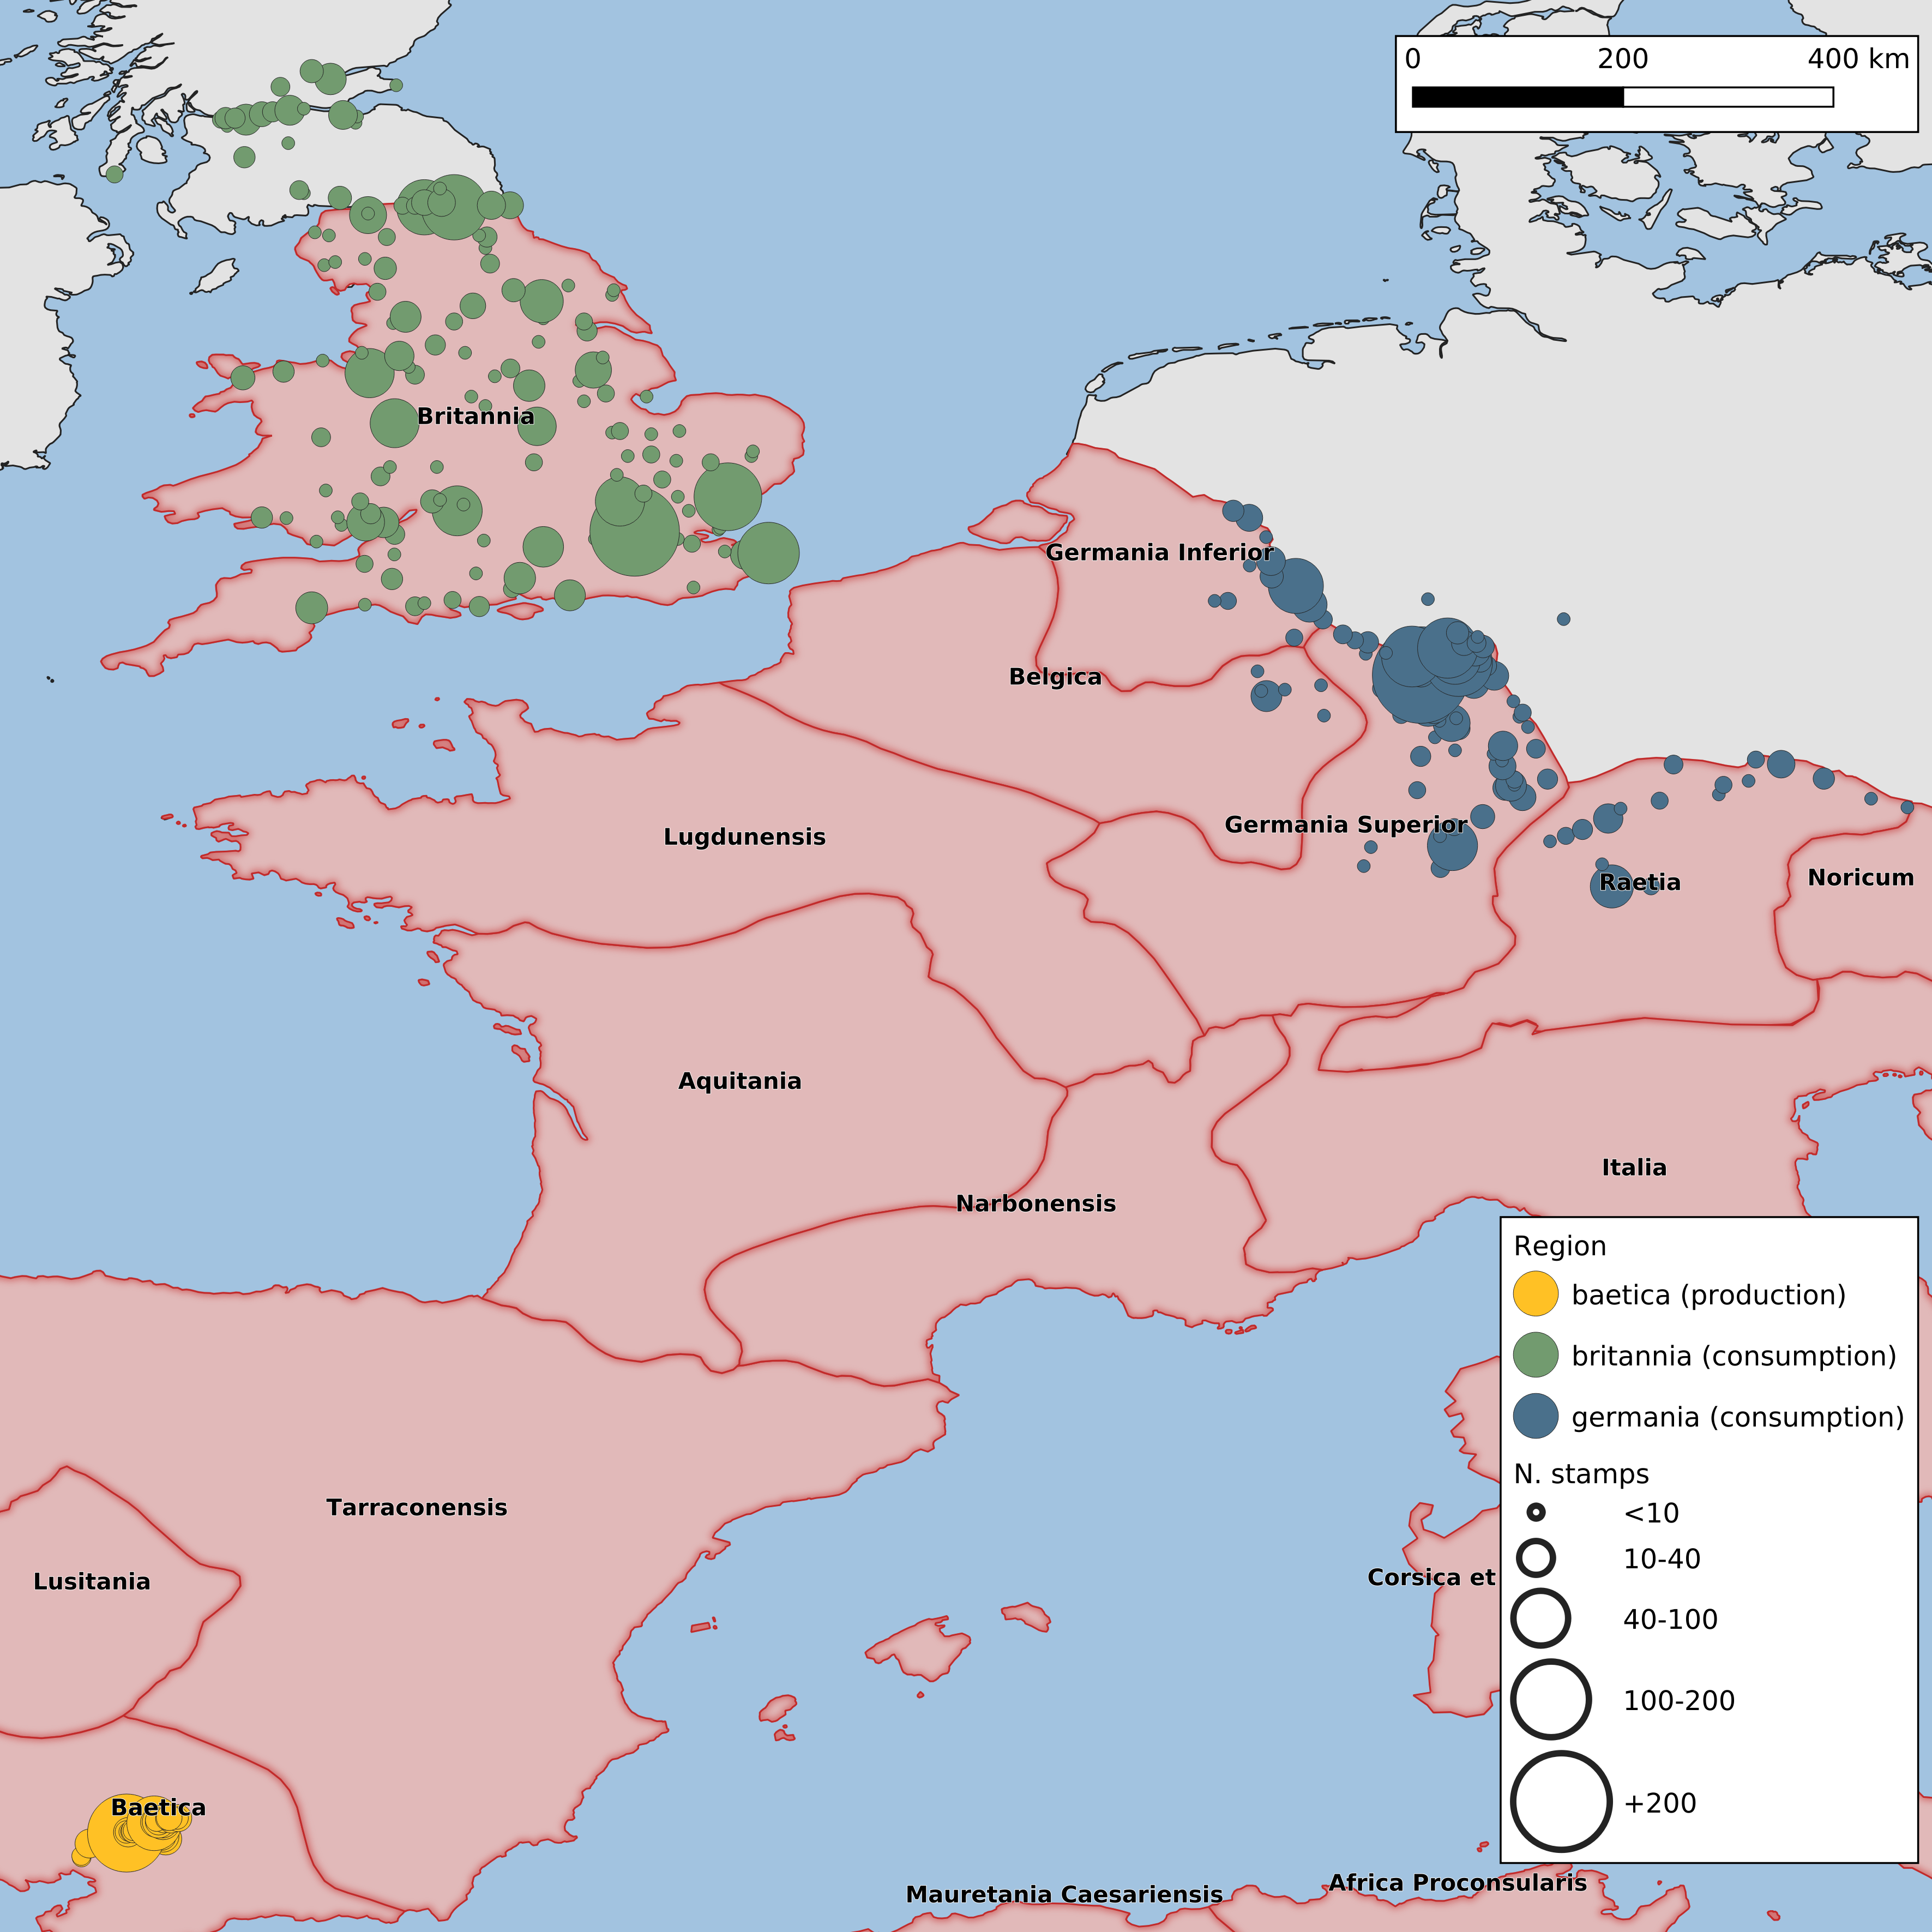
\includegraphics[width=\linewidth]{general_map}
\caption{Sites analysed in this paper. The colour defines the three different regions under study (\textit{Baetica} (yellow) as producer; \textit{Germania} (blue) and \textit{Britannia} (green) as consumers) while the size of each dot is proportional to the number of Dressel 20 amphoric stamps found on each site}

\label{general}
\end{figure} 
        
In \textit{Baetica} province we want to identify links between workshops based on the similarity of their stamps. In the consumption Roman provinces, our aim is to detect groups of nearby sites sharing stamps and to what extent stamps are clustered based on provinces. This economic connection could be identified with two ideas: a) nearby sites have more similar amphoric stamps and b) sets of stamps can only be found on specific provinces because they were shipped together.
%find in or find on

We proposed three working hypotheses based on these ideas: a) we can identify a correlation between spatial distance and the distribution of amphoric stamps, b) stamp sets found in nearby workshops should be more similar and c) there is low mobility of amphoric stamps from consumption centres to other regions (i.e. stamps always stay in the same region).

This study proposes a robust baseline to explore the distribution of Baetican olive oil production by identifying which centres have more similar stamps and then confront this measure against their proximity. To do this, a population-based approach has been used to analyse the dispersion of stamps between amphora workshops \citep{rubio-campillo_ecology_2018}. This quantitative method provides a way to measure the similarity between centre based on the amphoric stamps found on each of them. This ecological approach is based on three steps: a) to quantify stamp similarity between sites, b) to group sites based on this similarity and c) to find correlation patterns between stamp similarity and proximity. The rationale behind the method is as follows: if trade structure was centrally planned then we should be able to establish links between workshops and consumption sites based on the similarity of its stamps; if this is not the case then results would suggest that workshops worked independently and agreements were made at an individual level.

The paper addresses these questions, the analysis and results as follows: next section introduces the historical context. Section two defines the dataset and the methods used for the analysis. Section three presents the results and section four discusses them; the paper finishes with some concluding remarks on the research performed.

\section{The Amphoric production of Baetica}
\label{sec:1}

The \textit{Baetican} province was one of the most suitable regions to tackle the challenge of the huge demand for olive oil across the Roman provinces. For this reason, the area saw an increase in productivity as a massive specialised infrastructure of olive oil production was gradually deployed. This production of olive oil had the largest peak from the first to the third century AD~\citep{remesal_concierto}. 

Hundreds of presses and amphora-making workshops were built near a landscape covered by olive trees. These workshops made the amphorae which were filled with olive oil from the presses; they were built at the banks of the rivers Guadalquivir and Genil (see Fig.\ref{workshop}).

This proximity between production area, olive processing infrastructure, amphorae production and navigable rivers made the entire process extremely efficient. The strategic location allowed the transport of olive oil through riverine shipping towards the maritime routes that connected \textit{Baetica} with Mediterranean and Atlantic trade routes towards the rest of the Empire~\citep{garcia_vargas_enrique_formal_2010}.

\begin{figure}[htp]
	\centering
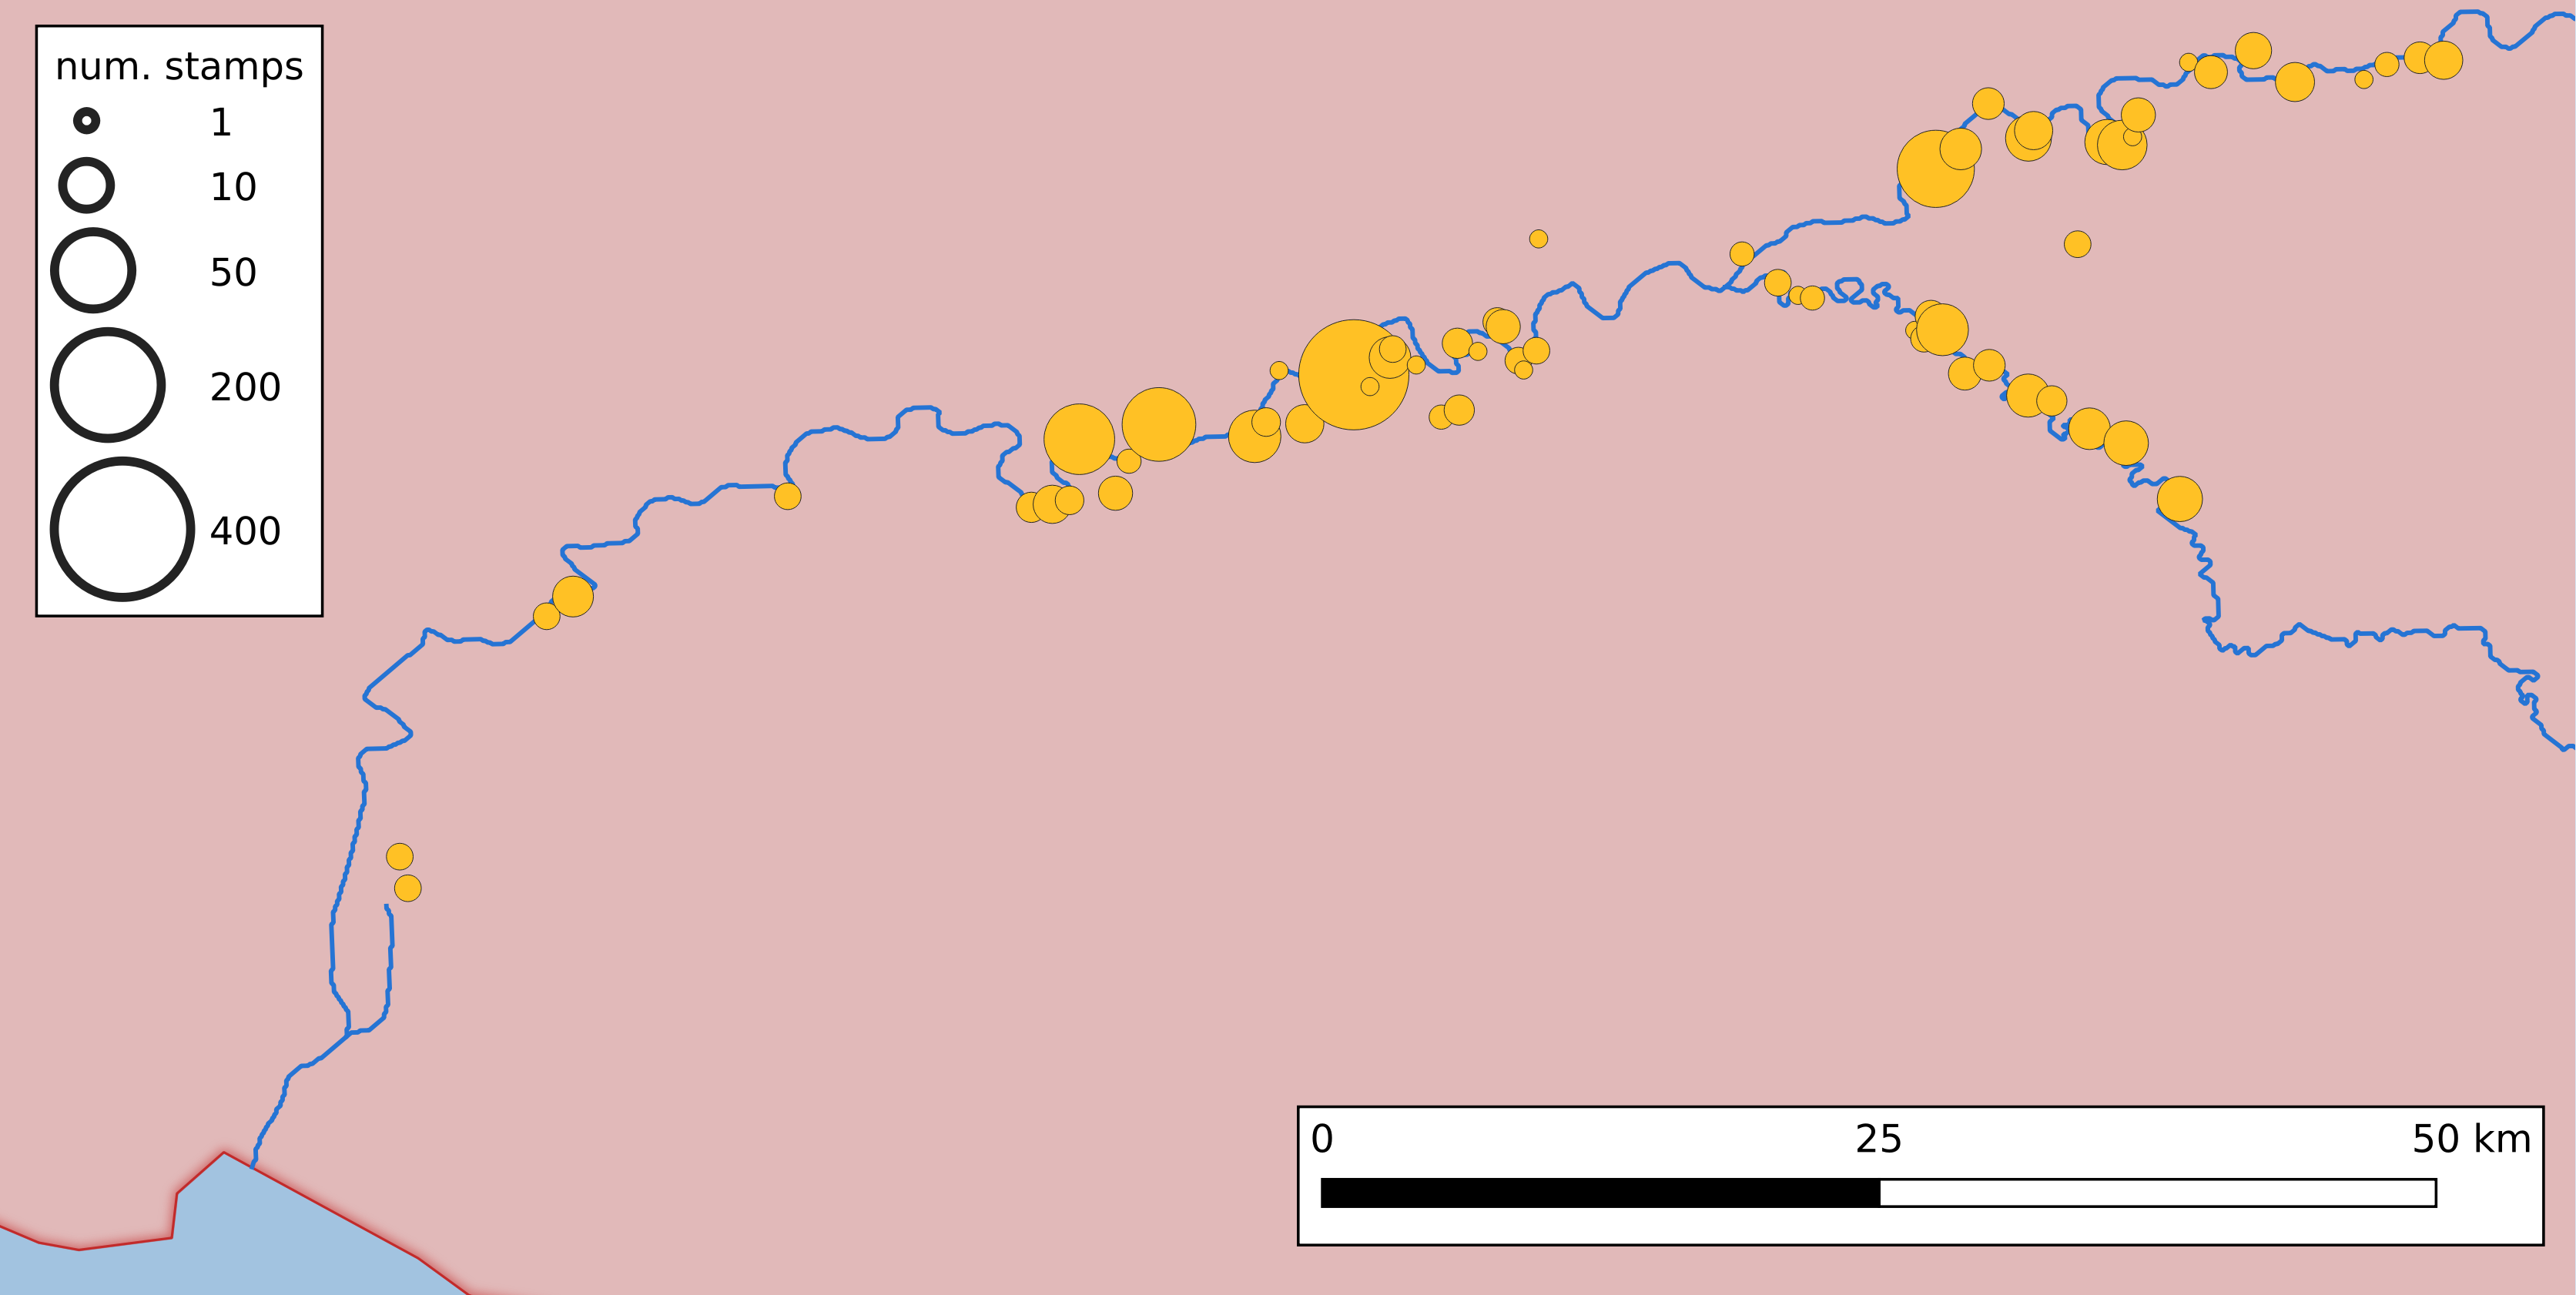
\includegraphics[width=\linewidth]{baetica}
\caption{Distribution of stamps found in Dressel 20 workshops along the Guadalquivir riverbank. The size of each point depends on the number of stamps found on each site}

\label{workshop}
\end{figure} 

The chronology of the Baetican workshops is typically defined between the first to the third centuries AD~\citep{millet_anforas_1998,rodriguez_baetican_1998,chic2005comercio}. Archaeological evidence suggests that this highly specialised production was developed across a long activity period\citep{remesal_anforas_2004}. The process seemed to have been planned at some level as is observed by the relatively minor changes in amphoric typologies and the high degree of standardisation in the production. 

The importance of this olive oil trade is revealed by the massive amount of Dressel 20 type amphorae found in all the Empire and particularly in the Western provinces~\citep{dressel_ricerche_1878,millet_anforas_1998}. This amphora has been commonly associated with the transportation of Baetican olive oil for supplying military camps and civil settlements~\citep{berni_millet_epigrafianforica_2008}. They have a recognisable globular form with a short neck and oval-shaped handles. Its capacity allowed to hold 70-75 litres of olive oil to be shipped and distributed throughout Empire \citep{berni_dressel_2016}.

Dressel 20 amphorae display a lot of interesting information beyond their shape, even though some of it is hard to interpret. A large percentage of Dressel 20 were marked with stamps, while some of them were also inked with \textit{tituli picti} or incised with \textit{graffiti}. The interpretation for most of these inscriptions is still open due to the fragmentation of the material, the lack of written records clarifying its use and for \textit{tituli} and \textit{graffiti} a small sample size of well-preserved elements~\citep{aguilera_evolucion_2007,rovira_guardiola_grafitos_2007}. 

\section{Amphoric stamps as a proxy for economic structures}
\label{sec:2}

Dressel 20 was the amphora most stamped during the Roman Empire~\citep[18]{millet_anforas_1998}. The large sample size of recovered Dressel 20 stamps is distributed across all Western provinces of the Roman Empire. This wide distribution is observed in the large volume of publications discussing the origin, use, chronology and spatial distribution of the stamped codes~\citep{dressel_ricerche_1878,rodriguez_economioleicola_1977,chicepi1985,millet_anforas_1998, remesal_sellar_2016} (Fig.\ref{amphora}).

\begin{figure}[htp]
	\centering
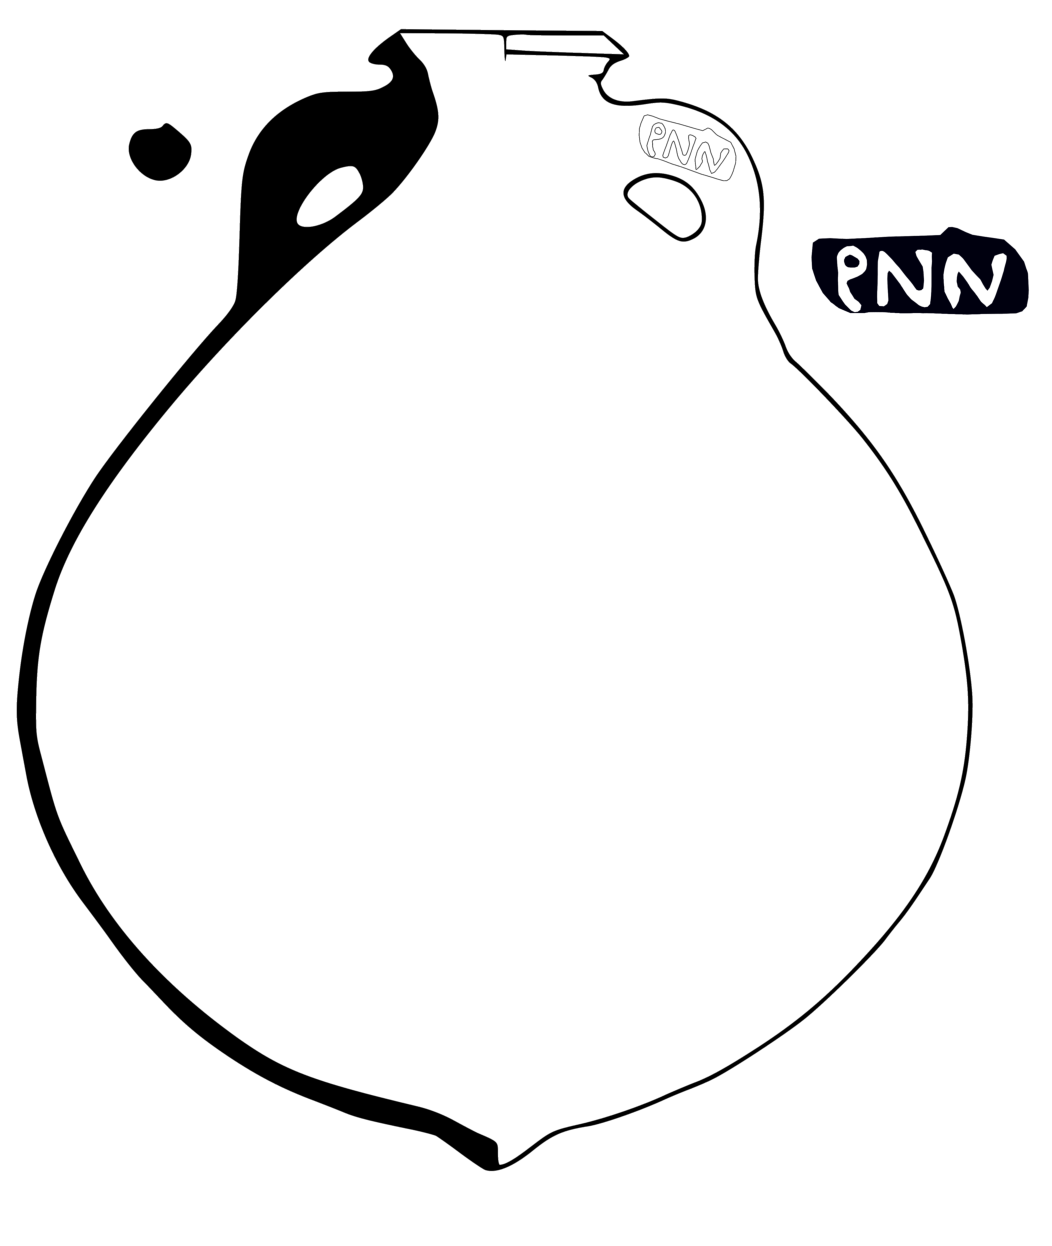
\includegraphics[scale=0.5]{dressel20}
\caption{Dressel 20 were typically marked with stamps of three letters called \textit{tria nomina}}
\label{amphora}
\end{figure} 
%found in find in
Most stamps seemed to have been used across a long activity period which can be difficult to date with the required level of accuracy. They have been frequently dated using as reference consular dates found on nearby \textit{tituli picti} recovered from \textit{Monte Testaccio}~\citep{Testaccio1, berni_millet_epigrafianforica_2008}.
The chronological information of \textit{tituli picti} is very useful, but the small amount of dates recovered and the fact that a vast majority of them come from the same site poses some challenges to this precise dating. In addition, the fact that \textit{Monte Testaccio} was a dump suggests that the disposition of amphorae vessels may have been altered at a later phase due to changes in the long-term dynamics of creation of this artificial mound.

The use of amphoric stamps can be a good proxy to explore the system of olive oil production and trade developed in \textit{Baetica} province. These stamps are typically found on handles but they could also be imprinted on rims and the amphora body~\citep{millet_anforas_1998}. The content information of the stamps was not defined by a single criteria, but they often displayed a code composed by letters and additional symbols. One of the most common forms is a code of three letters showing a \textit{Tria Nomina}~\citep{berni_millet_amphora_1996}; in this case the three letters are the initials of a Roman name. In some cases the full name may appear, while the meaning of other stamps is difficult to interpret~\citep{rodriguez_baetican_1998}. 

The stamp codes are interpreted based on three main ideas: content (olive oil), context (amphora workshop) and subject (individuals involved in the production). On the one hand, it seems that stamps could have been identified as the landowner of the olive groves \citep{rodriguez_economioleicola_1977}. On the other hand, they could also belong to the owner of the workshops where the amphorae were made or even to a group of amphora workers~\citep{berni_millet_epigrafianforica_2008}. Despite the unsolved question of ownership, some interesting ideas can be explored based on the finding of similar stamps across the Empire. Observable patterns can be used to explore how this production was organised and whether it is possible to identify specific production processes for olive oil trade. Our questions here will be focused on the distribution of amphoric stamps; were different stamps shipped through different distribution routes? Were specific stamp codes used in different workshops?

\section{Consumption centres: Britannia and Germania}
\label{sec:3}

The expansion of the Roman Empire to increasingly distant regions required an effort to intensify trade activity through Mediterranean and Atlantic routes. These needs effectively led to a gradual change in the economic and social structures as the trade networks that supplied the provinces and particularly the Roman army became more complex. An interesting example of this system is the figure of the \textit{praefectura annonae} which was created during Augustus's administration to organize wheat supply. The role of the \textit{praefectura annonae} was mainly focused on providing through \textit{frumentationes} a fixed monthly amount of wheat to each Roman citizen~\citep{remesal_annona_1986,remesal_concierto}.

Some authors argue elsewhere that this same \textit{praefectura annonae} could also have organised the supply of additional goods such as olive oil to the Roman legions~\citep{remesal_annona_1986,remesal_annona_1990}. From this perspective, olive oil supply seems to be particularly intense in militarised provinces that functioned as the borders of the Empire such as \textit{Britannia} and \textit{Germania}. The high percentage of Dressel 20 amphorae found in civilian sites close to the military garrisons also suggests the existence of diverse supply dynamics involving systematic trade between military sites to civil settlements~\citep{remesal_annona_1986, carreras_britannia_1998}. An explanation for the interest for exporting olive oil to the military garrison in the Roman provinces is still unclear. The reasons behind this effort to supply olive oil to all soldiers may be related to two aspects: a) consumption based on cultural reasons (i.e. social identification or habit  by a group of consumers) and b) economical and political reasons to create a redistributive system mechanism to supply military camps~\citep[69-70]{carreras_britannia_1998}. 

The Roman conquest of \textit{Britannia} and \textit{Germania} was a new opportunity to expand economical activity to support military efforts. High demand for olive oil in both provinces stimulated an important trade network involving different agents and the Empire itself. \textit{Baetica} became a strategic province for the production and distribution in both provinces as can be observed by the large volume of Dressel 20 amphora vessels found both in civil and military sites of these areas during and after the conquest. 

\subsection{Britannia}
\label{sec:4}

The evidence for olive oil consumption in \textit{Britannia} is scarce before the Roman conquest \citep{funari_corpus_1996,carreras_abastecimiento_2003}. The local population did not consume this product and it was not produced in the region as the landscape and climate of the British Isles was not suitable for the growth of olive trees~\citep[161]{monfort_britanniaen_1998}. Archaeological records suggest that this absence of olive oil changed with the arrival of a large amount of Dressel 20 amphorae to \textit{Britannia} from the first century A.D. onwards \citep{peacock_amphorae_1991,carreras_britannia_1998}. At this moment, we detect an increase of the olive oil exports linked to the arrival of legions caused by different military campaigns~\citep[161]{monfort_britanniaen_1998}. 

The increase of Dressel 20 exports created an important commercial network for exchanges. The demand for olive oil after the Roman conquest required of a new trade route due to the lack of local olive oil production; \textit{Baetica} was chosen as its main supply. This economic relation will be particularly intense for sites close to Hadrian Wall's garrisons. Olive oil production in \textit{Baetica} would cross the Atlantic until they reached the province and redistribute throughout the area from a series of strategic locations~\citep{carreras_atlantic_2012}.  This presence of Dressel 20 stamps in military camps in \textit{Britannia} has been widely studied in Roman archaeology \citep{williams_importation_1983,funari_corpus_1996,carreras_britannia_1998,carreras_abastecimiento_2003}. This intense consumption of olive oil also suggests the existance of provincial structures created to organise the supply of olive oil across military camps. There are no written records detailing how this redistribution of essential goods was organised in \textit{Britannia}, but the archaeological evidence suggests that cities may have been the central nodes of this local trade network~\citep{funari_economic_2005,orengo_seeds_2016}. 

The consumption of Baetican olive oil would experience a progressive slowdown from the third century A.D. onwards. This date matches a change in market strategy in the Empire. This gradual decrease on \textit{Baetican} olive oil exports can be observed as a decrease in the amount of Dressel 20 found in excavated sites as this typology is replaced by other types of amphorae from other places and particularly the African provinces~\citep{rodriguez1991aceite,millet_anforas_1998}.

\subsection{Germania}
\label{sec:4}

The distribution of Dressel 20 amphorae in the provinces of Germania Inferior and Germania Superior is not as well interpreted as the rest of provinces discussed in this work~\citep[293]{remesal_baetica_2002}. It is clear that there was a massive import of Dressel 20 in both provinces as is observed in archaeological excavations across the German \textit{limes}. However, it is still unknown to what extent trade agents participated in the distribution of Baetican olive oil in \textit{Germania} or the supply was exclusively focused on the Roman army garrisons\citep[156]{remesal_germn_2010}.

In any case, the introduction of olive oil in \textit{Germania} shows similar patterns than the one discussed for \textit{Britannia}. There is no archaeological evidence for olive oil consumption before the arrival of the Roman army to the region, while a majority of recovered Dressel 20 amphorae are located in the military sites built over the German \textit{limes} \citep{remesal_germaniaengl_2002}. The presence of the Roman army encouraged the exchange in the province as shown by the arrival of this product both civil settlement and military sites with a major concentration at the German \textit{limes}. It seems that some Baetican centres could have been assigned to a specific province for the olive oil supply to military garrisons~\citep[125]{remesal_concierto}. However, this hypothesis is hard to assess given the current lack of written evidence clarifying the meaning of the amphoric stamps. 

Some studies assumed that Roman naval technology was not suited for oceanic transport and for this reason defined riverine shipping across Rhône and Rhine rivers as the basic supply route for the German \textit{limes}. However, more recent large-scale computational analysis as well as new excavations on the Iberian Atlantic coast suggest that the Atlantic route, which was far more efficient, may have played a major role on the supply of \textit{Germania} and \textit{Britannia}~\citep{rubio-campillo_ecology_2018}.


\section{Material and Methods}
\label{sec:5}

The goal of this study is to explore these economic and long-range trade dynamics using amphoric stamps as proxies for common supply networks. We are especially interested on identifying links between Baetican production centres and consumption centres in the different \textit{limes}. 

For this analysis we used data collected in the CEIPAC database of amphoric epigraphy~\citep{remesal_centro_2015}. The CEIPAC dataset contains over 50.000 epigraphic records found on different types of amphorae (the database is openly accessible from \url{http://romanopendata.eu}). A large percentage of these records come from from \textit{Monte Testaccio}, but the rest is distributed mainly across the Western provinces of the Empire. It is worth mentioning that the database does not provide temporal information due to the reasons previously discussed, and for this reason this work can only analyze the spatial distributions within a coarse chronology of 2 centuries (3rd-1st AD).

In order to enable reproducibility of the results, this dataset as well as the source code are available on the following GitHub repository: \url{https://github.com/Mcotsar/Baetica\_stamps}.

\subsection{Production centres: Baetica province}
\label{sec:5}

We retrieved information on 3798 stamps found in Dressel 20 amphorae recovered from workshops within \textit{Baetica} province. Each record provides information about the spatial coordinates of the site and the inscribed code. Fragmented stamps or code not able to be read were discarded, thus finishing with a sample of 987 stamps from 81 sites and displaying 130 different codes.

Our dataset also contained a categorical variable defining the \textit{conventus} for each production site. The \textit{conventus} were administrative centres for territorial organisation under the Roman Empire \citep[58]{ozcariz_gil_administracion_2013}. The creation of the \textit{conventus} in some Roman provinces was a form of control with the purpose of organising provincial administration~\citep{albertini_les_1923}. The production area for Dressel 20 amphorae extended across three different \textit{conventus}: \textit{Hispalensis} (currently Seville, hereafter \textit{Hispalis}), \textit{Cordubensis} (currently C\'ordoba, hereafter \textit{Corduba}) and \textit{Astigi} (currently \'Ecija, Sevilla, hereafter \textit{Astigi})~\citep{rodriguez_economioleicola_1977,chicdatos2001,berni_millet_epigrafianforica_2008} . 

%3798 = base de datos sin limpiar
%3791 = base de datos limpiada con cleanstamp.py
%3787 = no sé a qué corresponde pero es archivo baetica.csv

It is worth mentioning that some workshops were coded under the same geographical coordinates. For instance, the stamps of two nearby amphora workshops such as Tesorillo de Do\~na Mencia and Do\~na Mencia were catalogued under different names while sharing the same geographical coordinates. The interpretation of our analysis considered this bias in the archaeological dataset which may have a minor effect in the final results. 

The first step of this analysis was to compute the frequency distribution of stamp codes and analyse it using Exploratory Data Analysis (EDA). This would allow us to study the distribution of the stamps across centres as can be seen in Figure~\ref{stamps}. As can be seen the distribution is widely diverse with most workshops having only one stamp, while a few workshops contained over 100 stamps. Particularly, one workshop (La Catria) concentrated a large percentage of the amphoric stamps with a total number of 228 stamps.

This uneven distribution of stamps is typical for amphora production as it is observed that a major concentration on the number of stamps is focused on a few workshops~\citep{coto-sarmiento_identifying_2018}.

\begin{figure}[htp]
	\centering
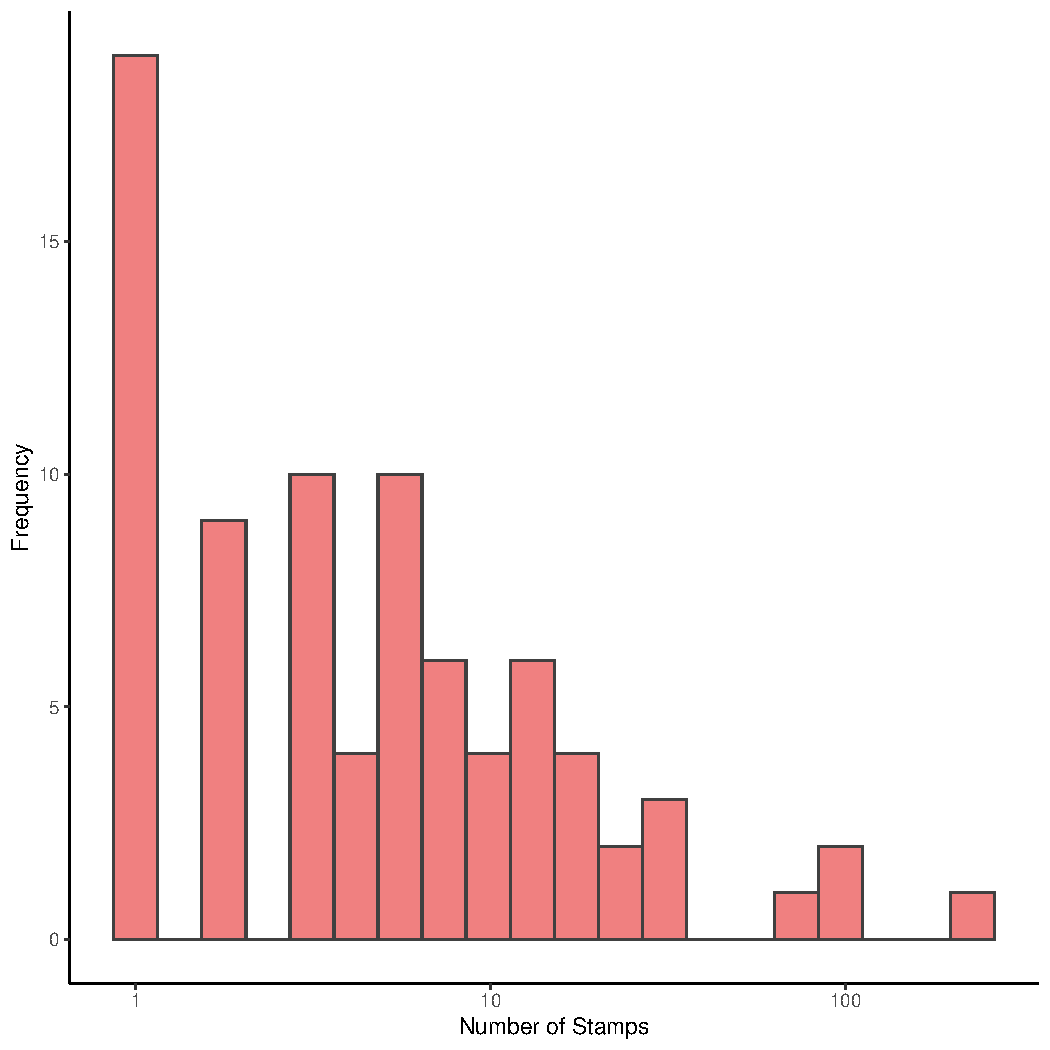
\includegraphics[width=\linewidth]{frequencystamp.pdf}
\caption{Histogram of stamps found in different workshops. Y axis shows the number of workshops where a given number of stamps have been found (X Axis). X axis is shown at a logarithmic scale given the long right tail}
\label{stamps}
\end{figure} 

The distribution of codes in stamps for each \textit{conventus} can be seen in Figure~\ref{frequency}. The majority of stamps are concentrated in \textit{Hispalis} (574 stamps) while \textit{Corduba} and \textit{Astigi} have roughly half this number (267 and 146 stamps respectively). The workshops of the three \textit{conventus} show a similar pattern on the stamp frequency distribution with the exception of 2 large workshops in \textit{Hispalis} (La Catria and Arva). On these two workshops a comparatively large amount of stamp codes were found (29 different codes on each of them). According to previous studies, those workshops became the most important centres of amphora production in the region \citep{rodriguez_economioleicola_1977,arva_1997}.

It is worth mentioning that a majority of these stamps were collected during field surveys while only a hanfdul of workshops have been excavated; this may explain some of the differences in sample size as there could be intensity bias across the different sites~\citep{arva_1997}.
 
\begin{figure}[htp]
	\centering
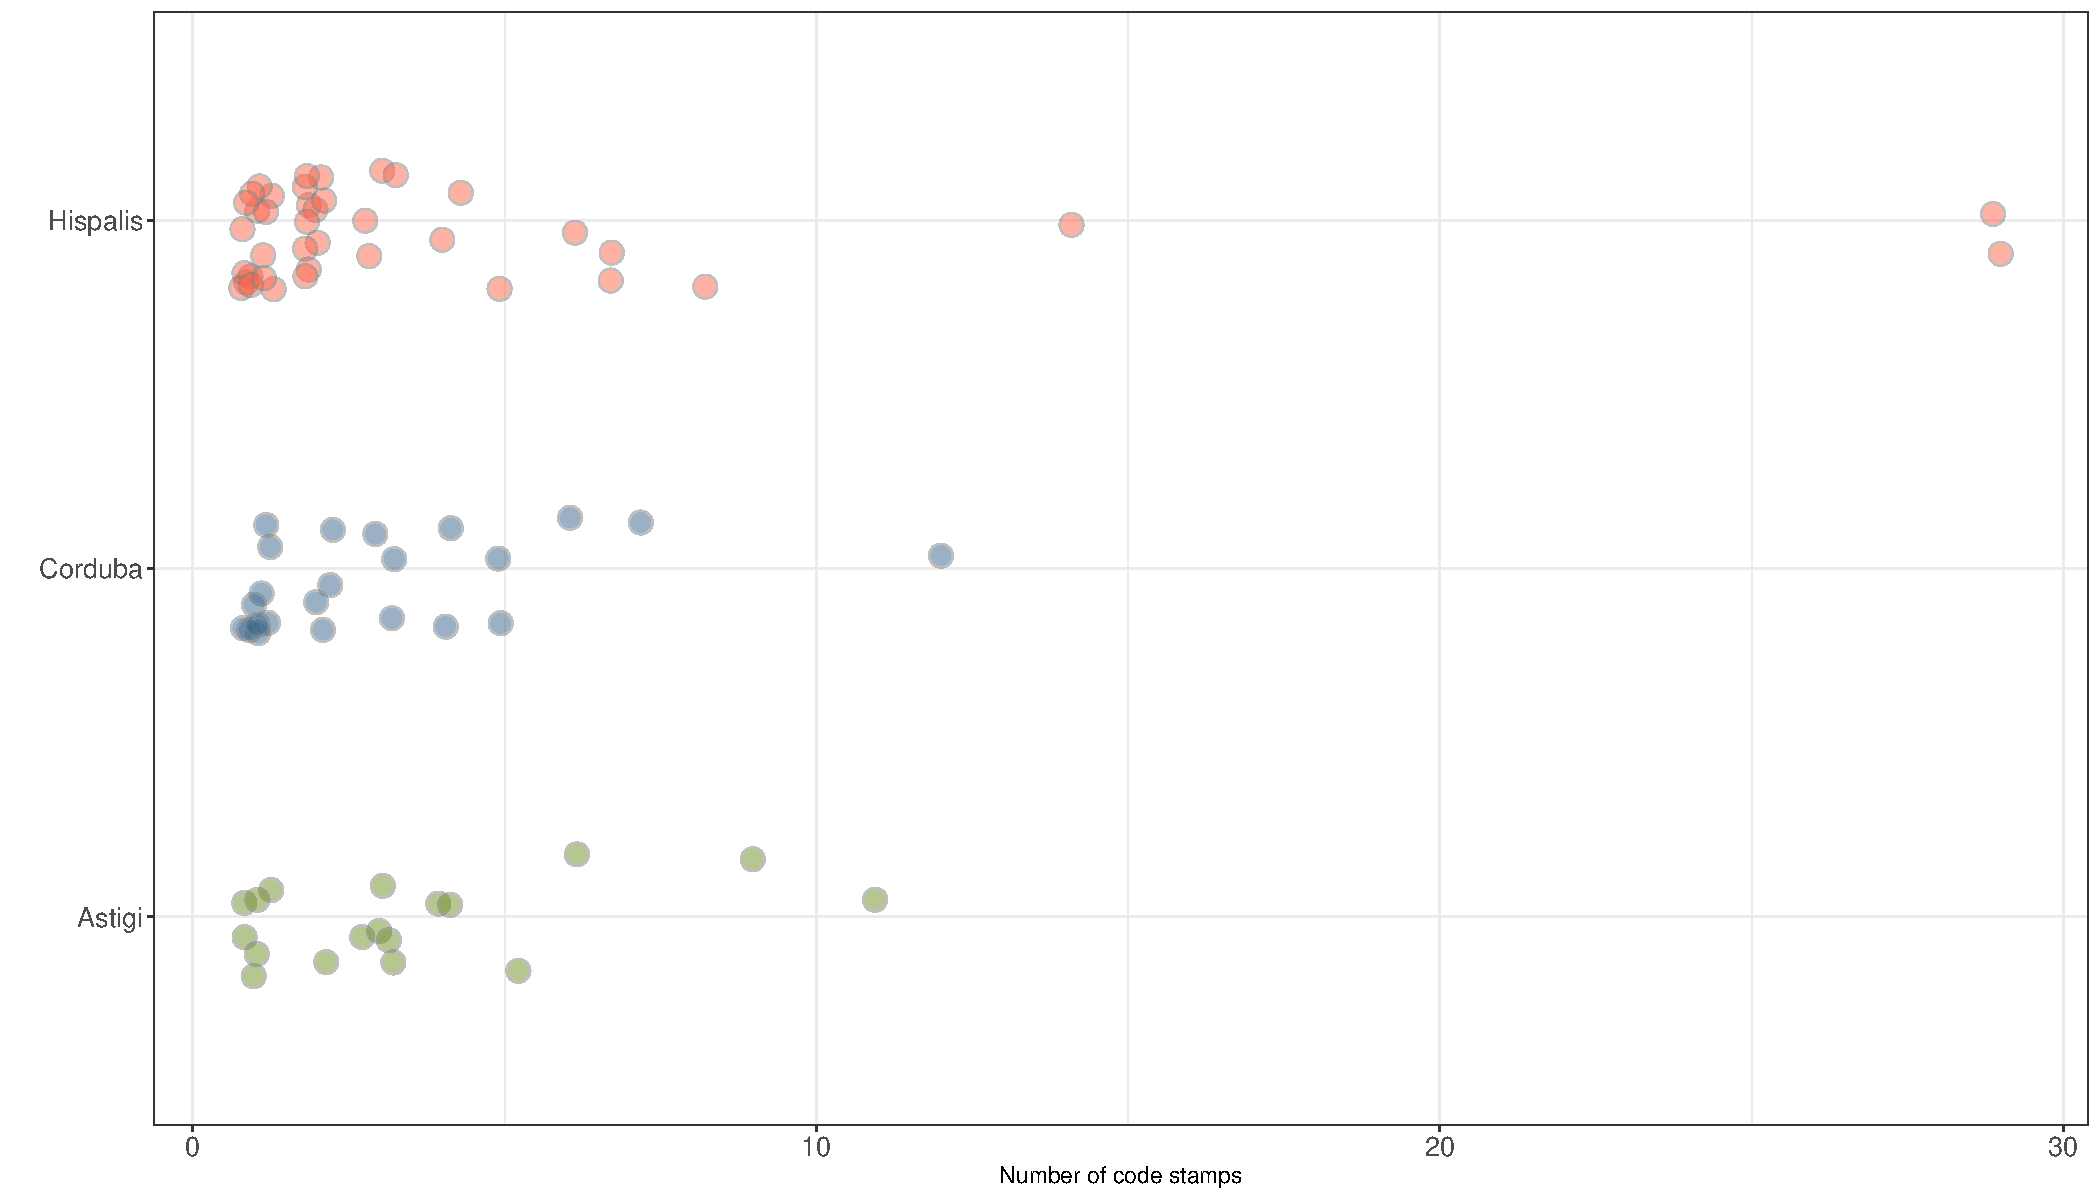
\includegraphics[width=\linewidth]{frequency}
\caption{Distribution of the number of different codes in stamps (X axis) for each \textit{conventus} (Y axis). Each dot corresponds to a workshop. Colours are represented by areas divided into \textit{Hispalis} (red), \textit{Astigi} (green) and \textit{Corduba} (blue)}
\label{frequency}
\end{figure} 


\subsection{Consumption centres: Britannia and Germania}
\label{sec:5}

The analysis of stamps in consumption areas also used the CEIPAC database and filters performed for the previous dataset. However, in this case there was a large amount of sites with only one or two stamps which may introduce noise in the similarity analysis. This is the reason why in this case an additional filter was performed and we only selected sites having at least five stamps.

The output was a dataset of 3386 stamps with similar sample size: 1765 from \textit{Britannia} and 1621 for the \textit{Germania} provinces. Both \textit{Germania} and \textit{Britannia} were analysed as frontiers and not as administrative Roman provinces; we included in the sample some centres that are actually located beyond the administrative boundaries but were considered part of the same border. Specifically, for the German \textit{limes} we included sites from the two provinces (Superior and Inferior) while the analysis of \textit{Britannia} extended to \textit{Caledonia}.
 
%We analysed a dataset of 2219 stamps from different centres in \textit{Britannia}. 
%CITAR (Callender, 1965; Carreras Monfort y Funari,1998; Ayllón-Martı́ et al., 2018). 
The 1765 stamps from \textit{Britannia} showed 986 unique codes from 46 sites. These consumption centres can be seen in Figure~\ref{britannia}.
 
\begin{figure}[htp]
	\centering
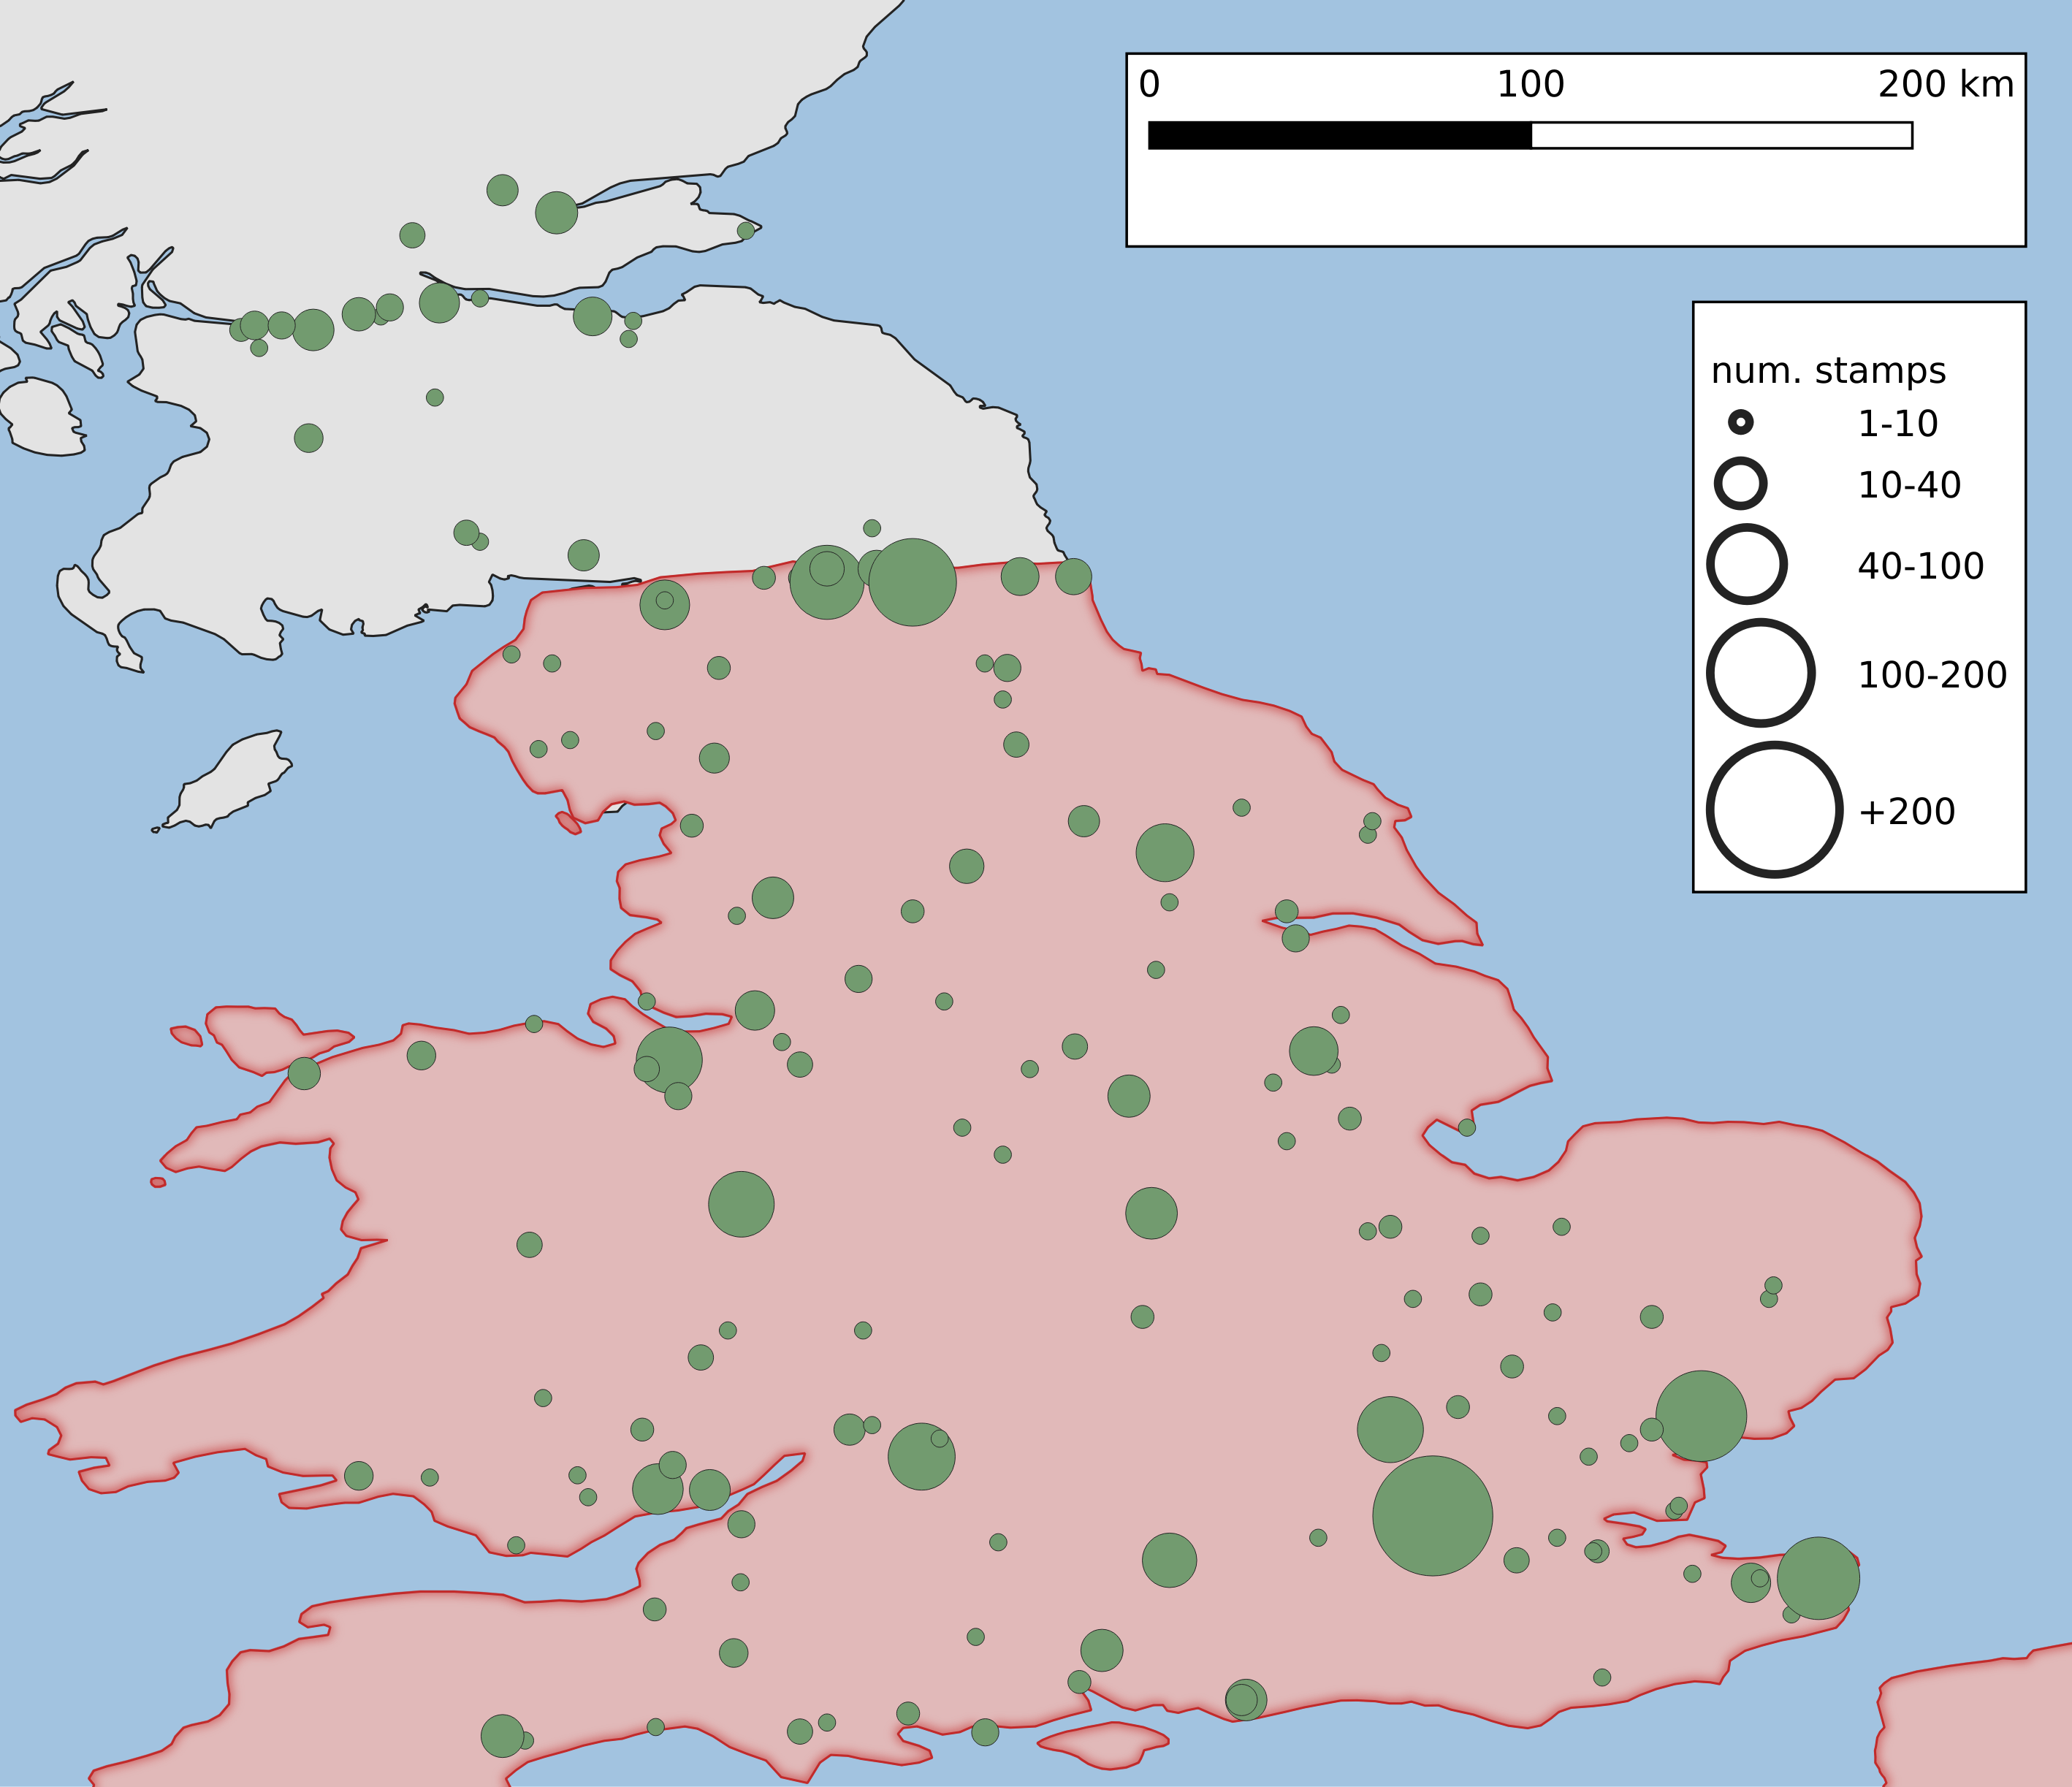
\includegraphics[width=\linewidth]{britannia}
\caption{Sites in \textit{Britannia} where Dressel 20 amphoric stamps have been found. Each dot is a site while its size shows the sample size of stamps found on the site. A majority of stamps have been found in garrisons related to Hadrian's and Antonine walls}
\label{britannia}
\end{figure} 

The 1621 stamps from \textit{Germania} displayed 850 different code from the same number of sites (46) which can be seen in Figure~\ref{germania}.

\begin{figure}[htp]
	\centering
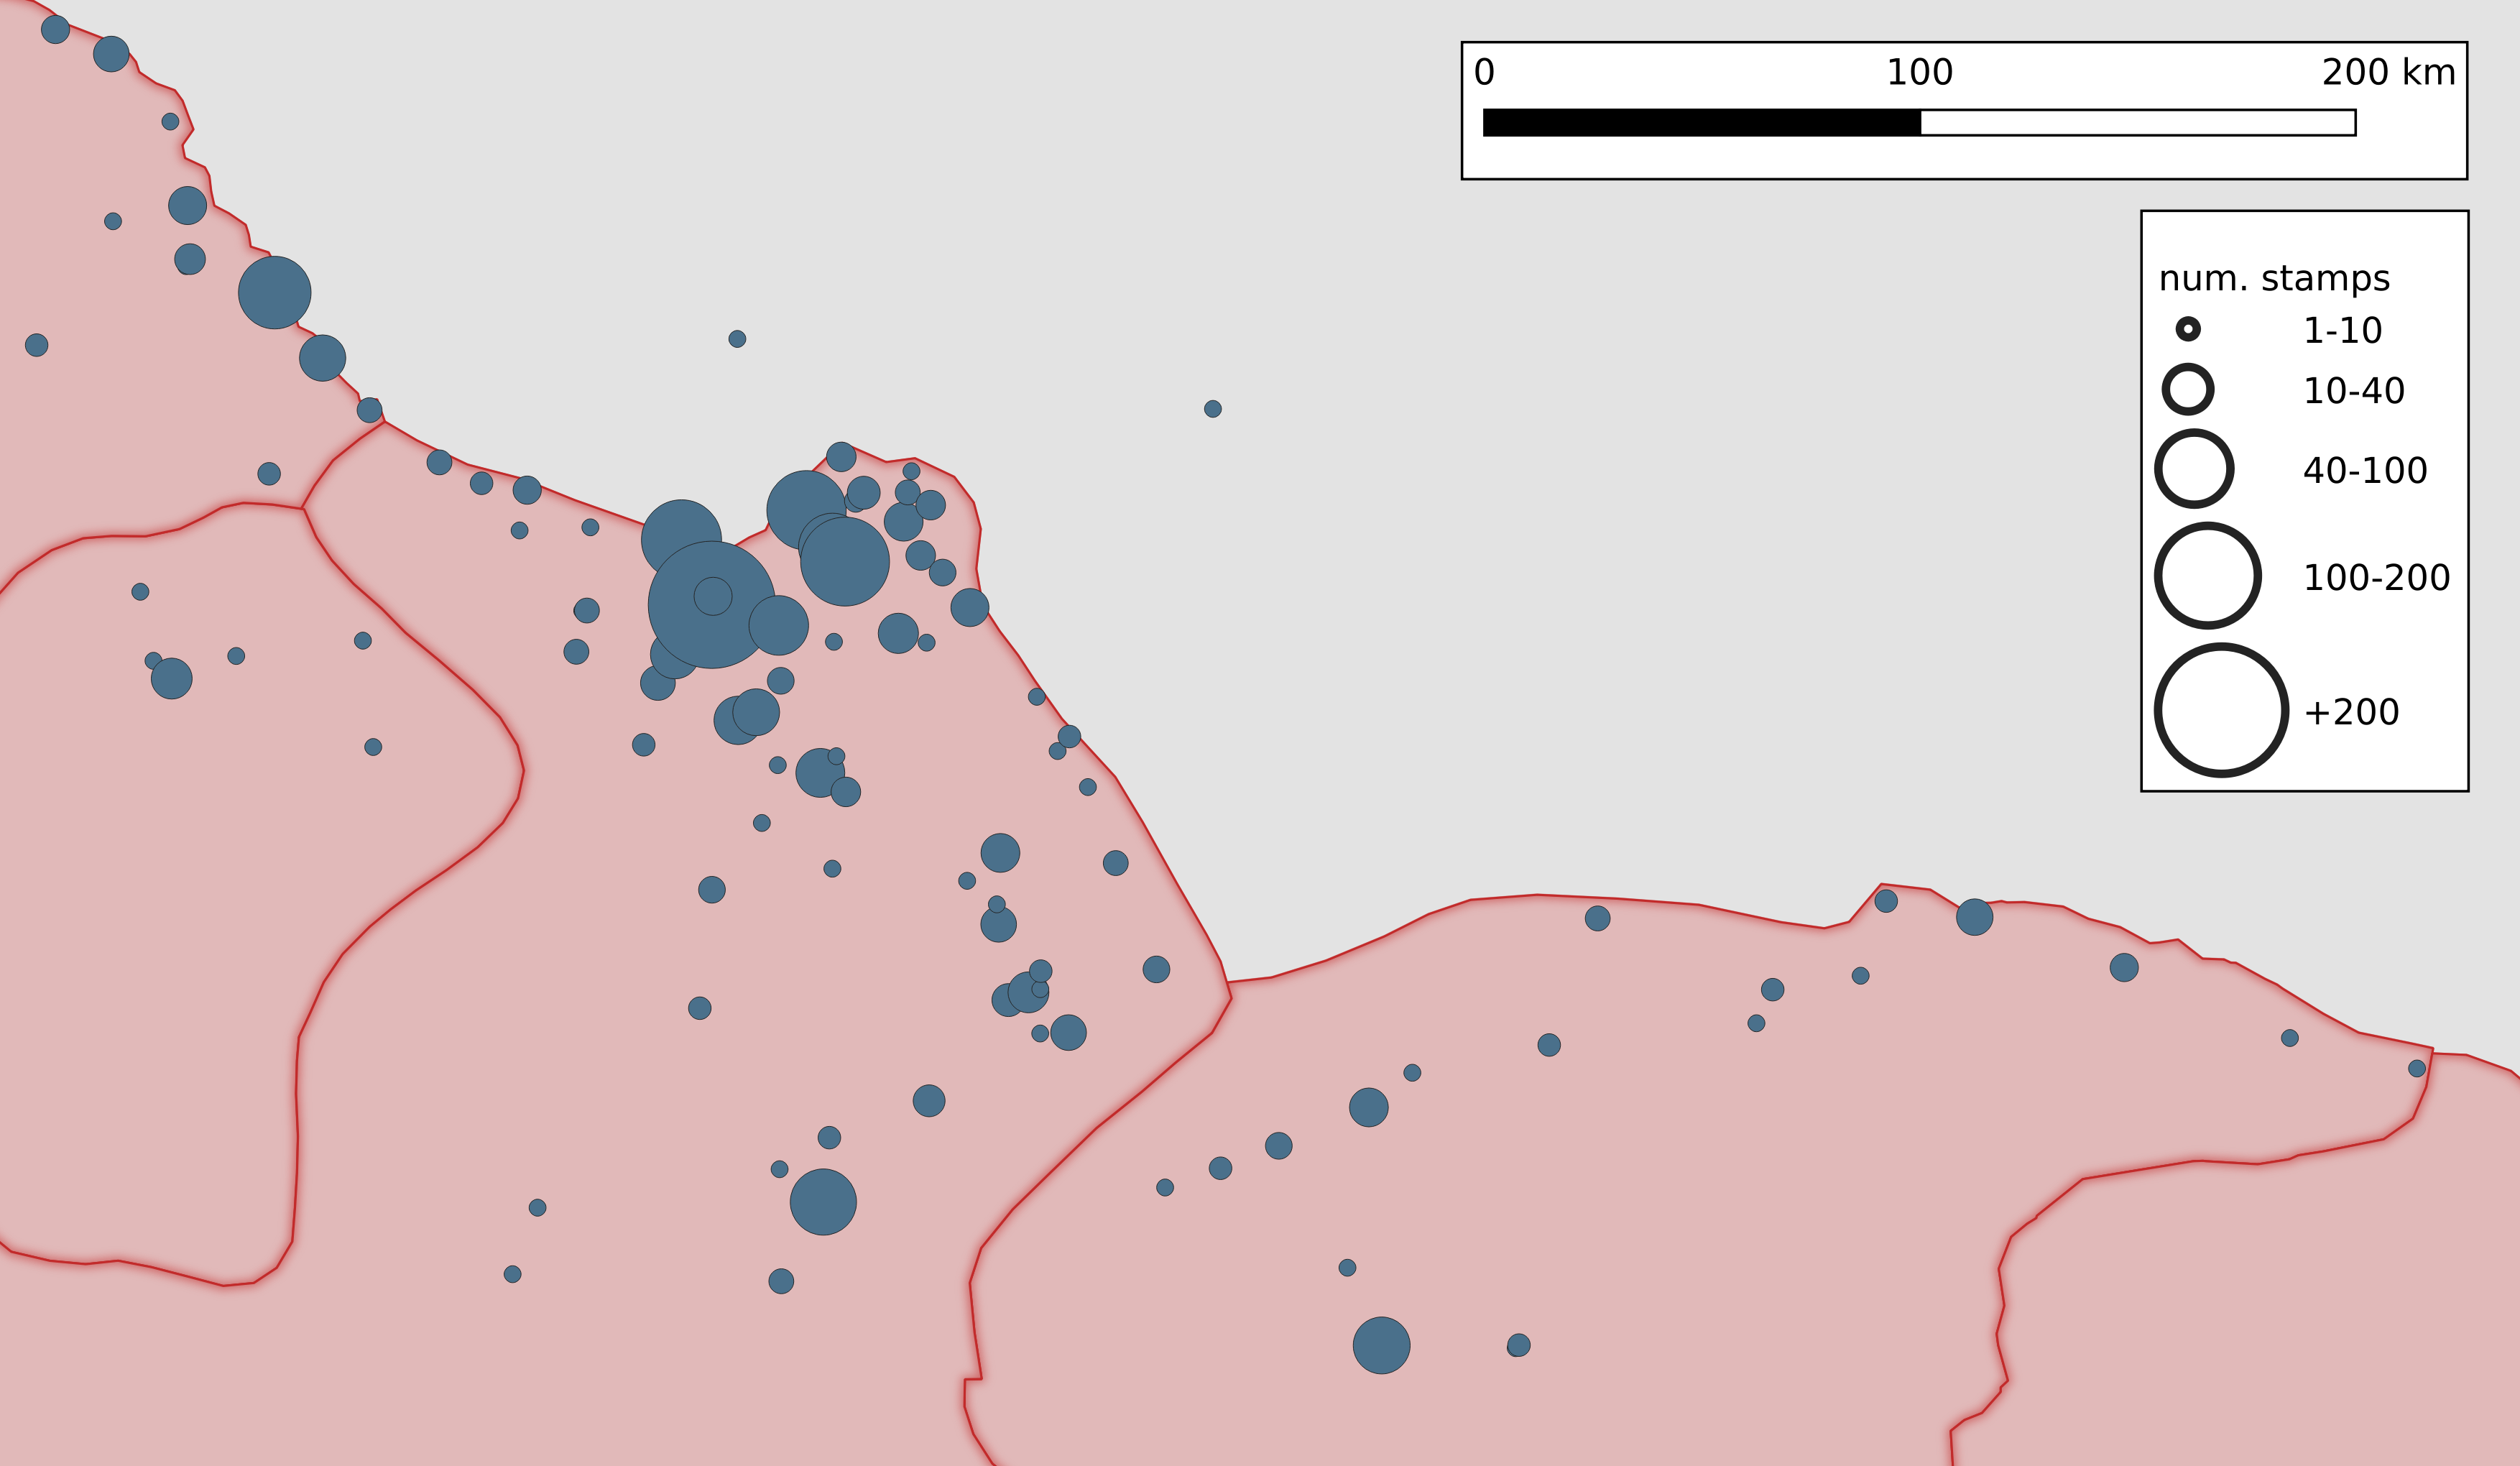
\includegraphics[width=\linewidth]{germania}
\caption{Sites in Germania where Dressel 20 amphoric stamps have been found. Each dot is a site while its size shows the sample size of stamps found on the site. Most sites are located along the German \textit{limes}}
\label{germania}
\end{figure}

\subsection{Quantifying similarity}
\label{sec:5}

Similarity between amphora workshops and/or consumption sites was measured by quantifying a distance (also called dissimilarity) between the set of stamp codes found for each pair of sites (i.e. to what extent the stamp codes found on these sites were different). The chosen measure for this study was the Morisita-Horn index \citep{morisita_measuring_1959, horn_measurement_1966}. This method was applied to measure the dissimilarity between different samples of stamps while taking into account the frequency that each code is present on each site. Generally, it describes the dissimilarity between the system of two communities based on the idea of inverse correlation between diversity and species \citep{magurran_why_1988}. In our case, stamps from different sites will be used as a proxy to measure their dissimilarity by analysing their code. 

The formula can be described as follows \citep{magurran_measuring_2013}:

\begin{equation}
D(MH) = 1- \frac{2 \sum(a_{i} \cdot b_{i})}{(d_{a} + d_{b}) \cdot (N_{a} \cdot N_{b})}
\end{equation} \\

$d_{a}$ and $d_{b}$ are given by the following equation:

\begin{equation}
d_{a} = \frac{\sum a_{i}^{2}}{N_{a}^{2}} 
\end{equation} \\

where $N_{a}$ is the total number of stamps found in workshop A; $N_{b}$ is the total number of stamps found in workshop B; $a_{i}$ is the number of different stamps for workshop A and $b_{i}$ is the number of different stamps for workshop B.

Considering our dataset as a non-uniform sample, this method provides a useful tool to handle large samples with different sizes and diversity \citep{wolda_similarity_1981}. Morisita-Horn index gives a distance value between 0 (sites have exact stamp codes and frequency distribution) and 1 (complete difference between stamp codes). To apply Morisita-Horn index, we first calculated the number of times that each stamp code appeared in an amphora workshop. 
This method allowed us to bear in mind the number of frequency of stamps for each workshop. For example, if two workshops had similar stamp code distribution then the distance index would be close to 0 whereas sites with no overlap between stamp codes would give a distance close to 1.

\subsection{Hierarchical clustering}
\label{sec:5}

Morisita-Horn was used to generate a pairwise matrix of distances between sites based on the overlap of the amphorae stamp codes recovered from them. Hierarchical clustering was then applied to this matrix in order to group sites based on the distance of their stamp codes. The construction of this similarity tree would allow us to analyse the relationship between groups of sites and the distribution of similar stamp codes. The results were visualised using a dendrogram to identify patterns within the different clusters.

\section{Results}
\label{sec:6}

\subsection{Production centres: Baetica Province}
\label{sec:6}

The result of the hierarchical clustering inferred from Morisita-Horn measures can be seen in Figure~\ref{dendro}. This visualisation suggests that most amphora workshops used a single stamp code which has not been found in any other site. Simultaneously the majority of stamp codes found on multiple sites are only present in two or three workshops. The combination of these two patterns generates a map of low similarity values for the entire sample.

Nearby workshops seem to display a higher similarity than distant workshops and the higher degrees of similarity between sites could be related to their spatial closeness; additionally, the workshops with higher similarity values belong to the same \textit{conventus} area, such as Picachos, Cerro de los Pesebres and El Castillejo.

%\begin{sidewaysfigure}[htp]
\begin{figure}[htp]
	\centering
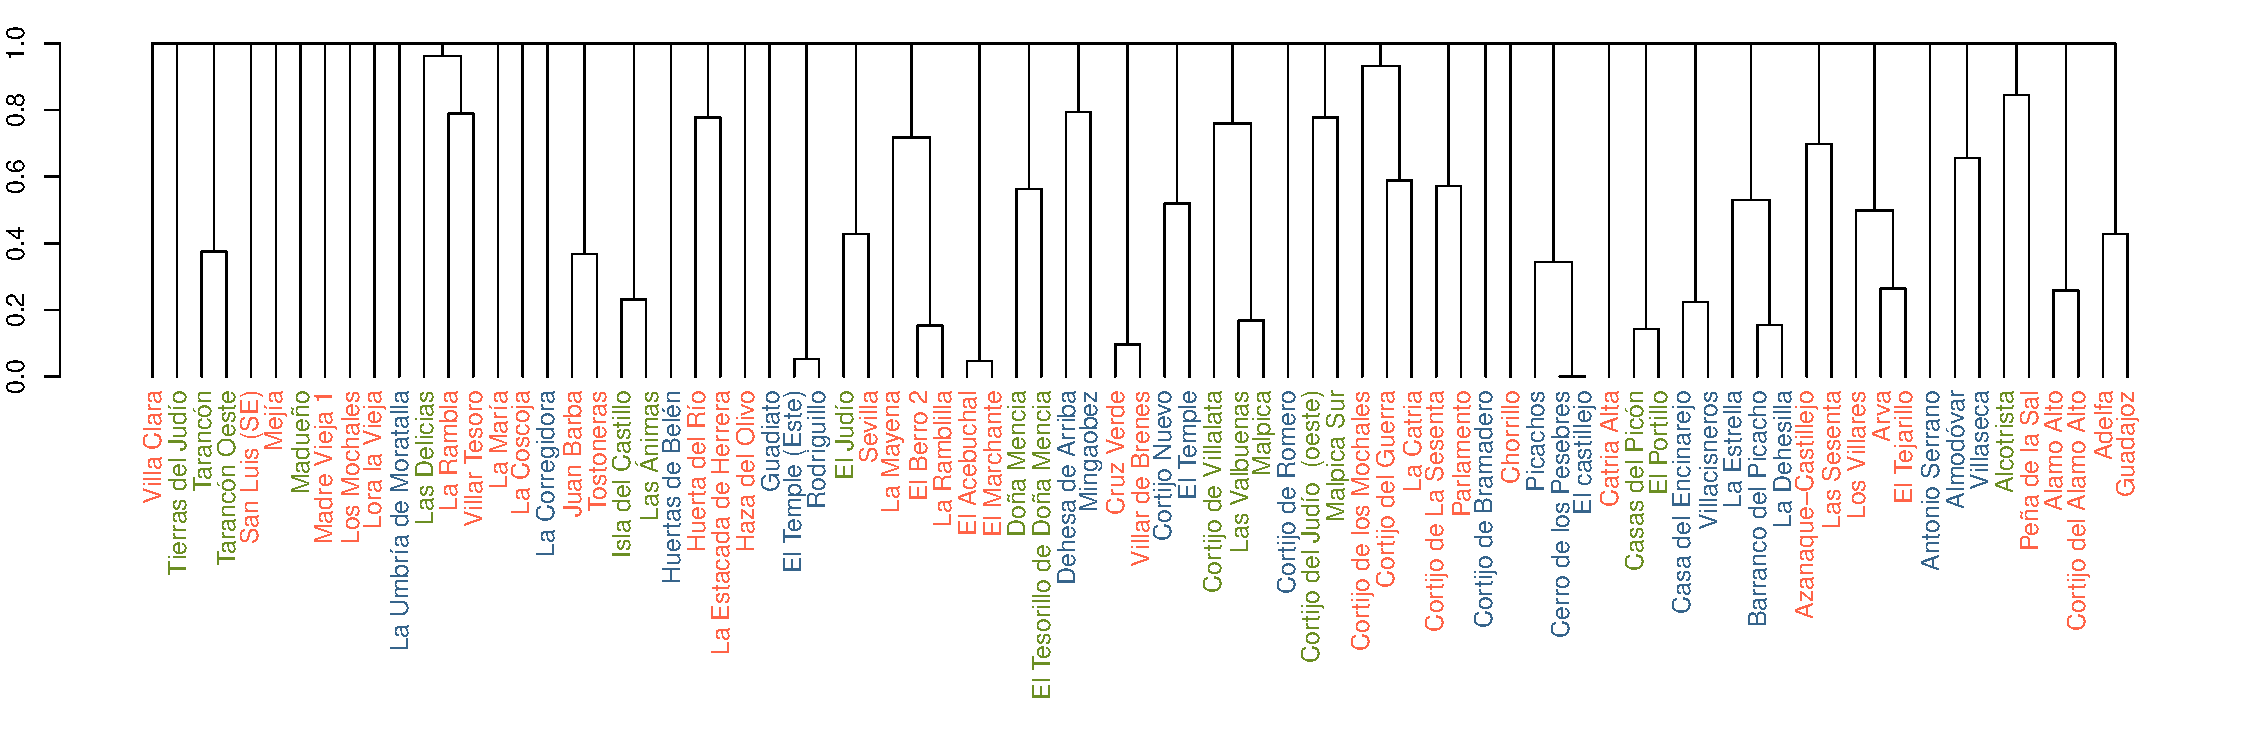
\includegraphics[angle=270, width=0.7\linewidth]{dendro}
\caption{Dendrogram displaying hierarchical clustering of \textit{Baetican} Dressel 20 workshops based on Morisita-Horn metrics. Site names are colour-coded by \textit{conventus}: \textit{Hispalis} (red), \textit{Astigi} (green) and \textit{Corduba} (blue)}
\label{dendro}
%\end{sidewaysfigure}

\end{figure}

\subsection{Consumption centres: Britannia and Germania}
\label{sec:6}

Results for the consumption regions display similar patterns than the ones found in the production area of \textit{Baetica}. The most significant difference is the lower similarity values as can be seen in Figure~\ref{britmap}.


%\begin{sidewaysfigure}[htp]
\begin{figure}[htp]
	\centering
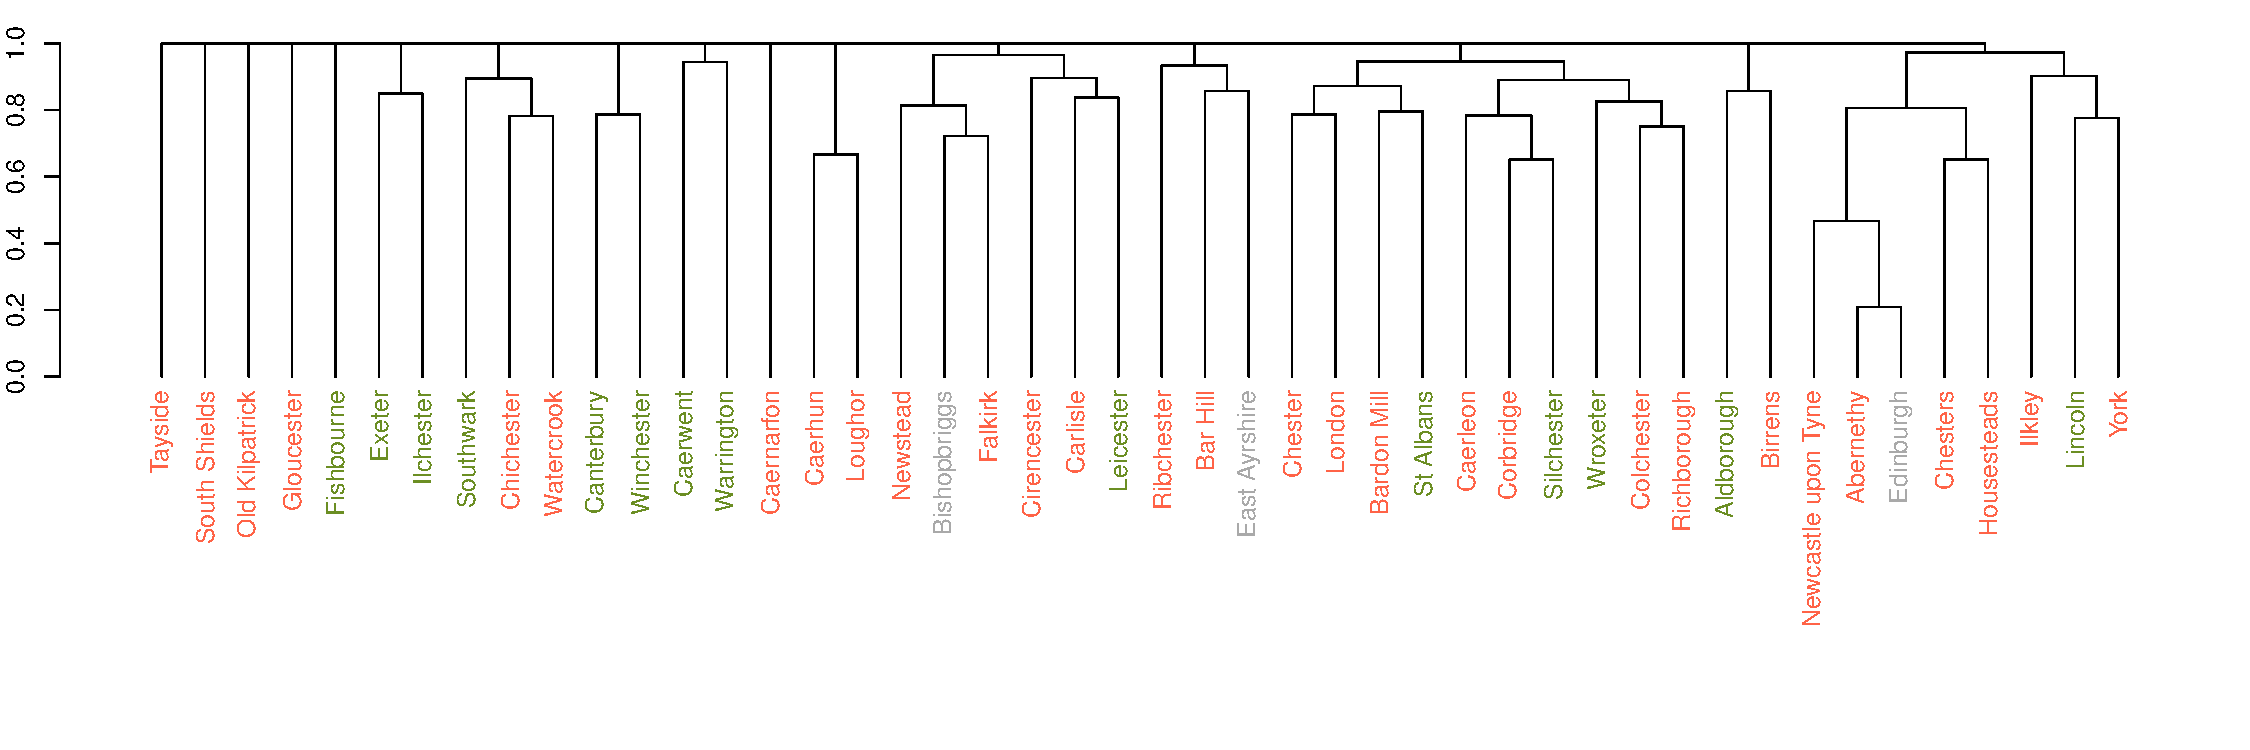
\includegraphics[angle=270,
width=0.7\linewidth]{dendrobrit5.pdf}
\caption{Dendrogram displaying hierarchical clustering for \textit{Britannia} sites based on Morisita-Horn metrics. Site names are colour-coded by typology: military sites (red), civilian sites (green) and unspecified (grey)}
\label{britmap}
%\end{sidewaysfigure}
\end{figure}

The lower similarity of stamp codes in \textit{Britannia} compared to \textit{Baetica} could be explained by a change of scale as the area under study is much bigger and the sites are more distant between them. The pattern can be more clearly observed for military sites which are often more well researched; in this case the ones with higher similarity tend to be geographically closer. To summarize, the same patterns than before can be observed on the dendrogram: 1) nearby sites tend to share more similar stamps and 2) a majority of stamp codes are only found in one site.
 
The similarity of sites based on Dressel 20 stamp codes is also low in \textit{Germania} as can be seen in Figure~\ref{germap}. 

%\begin{sidewaysfigure}[htp]
\begin{figure}
	\centering
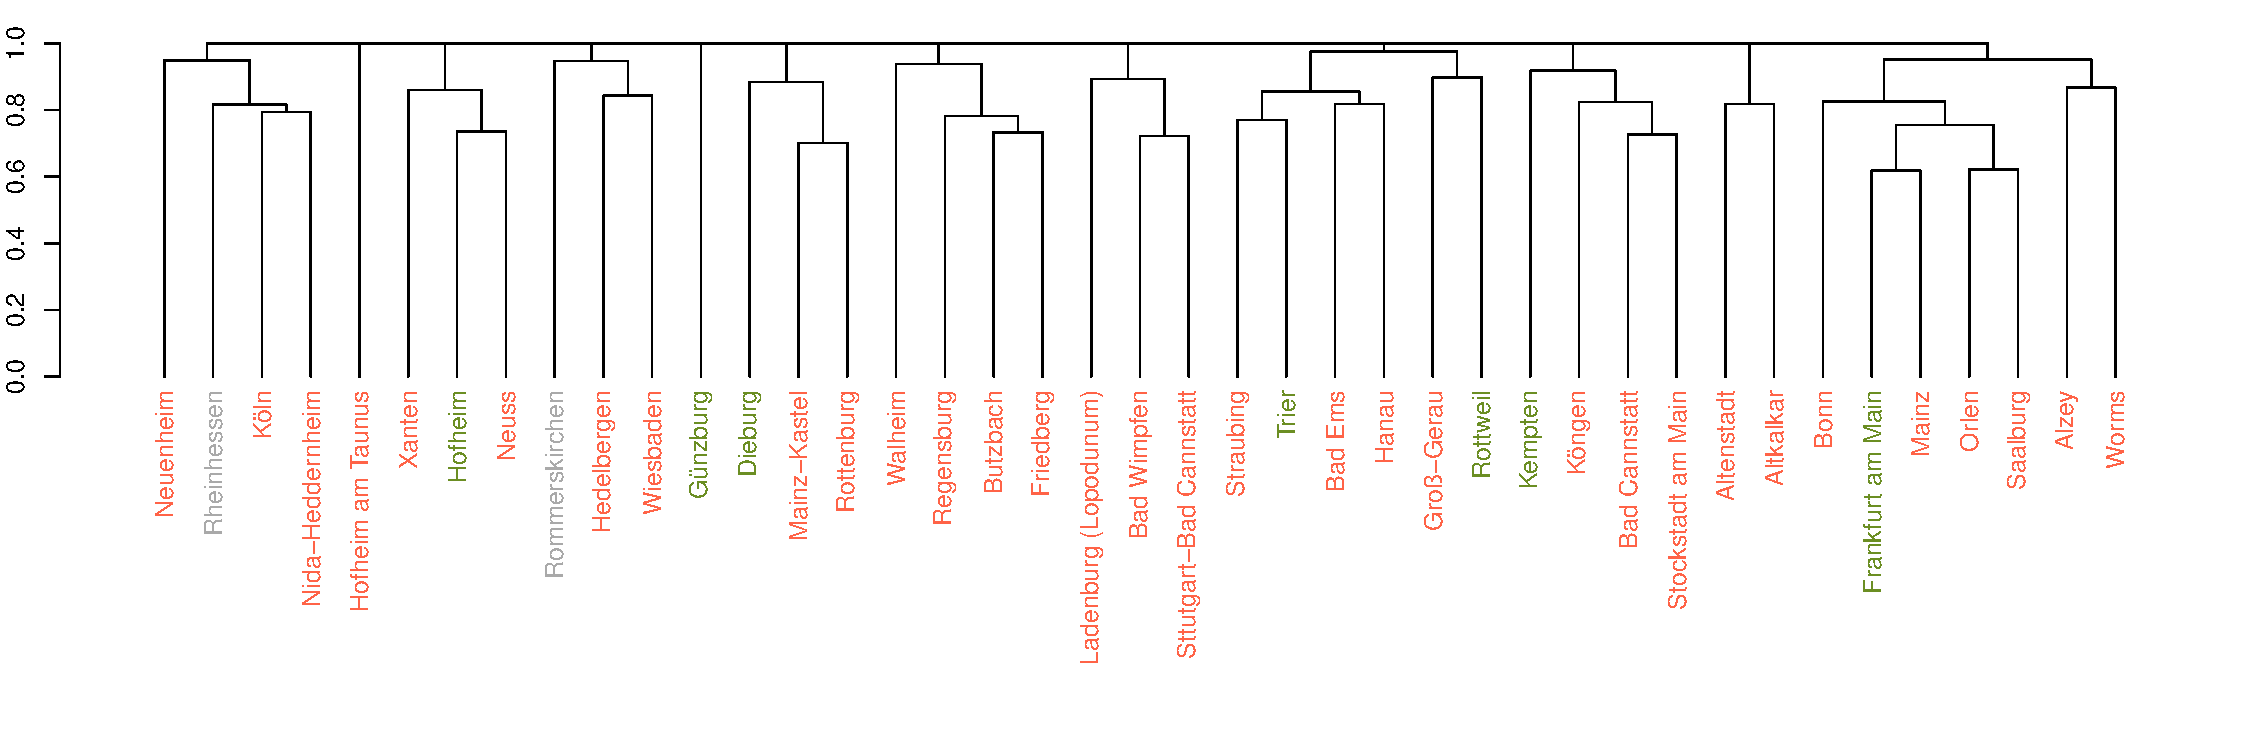
\includegraphics[angle=270, width=0.7\linewidth]{dendroger5.pdf}
\caption{Dendrogram displaying hierarchical clustering for \textit{Germania} sites based on Morisita-Horn metrics.  Site names are colour-coded by typology: military sites (red), civilian sites (green) and unspecified (grey)}
\label{germap}
\end{figure}
%\end{sidewaysfigure}

Again, results in \textit{Germania} exhibit similar patterns with lower similarities. The only difference is that a higher concentration of sites sharing similar stamps was found in militarised areas near the \textit{limes}.


\section{Discussion}
\label{sec:7}

This work has explored to what extent the distribution of amphoric stamps can provide insights into the organisation of olive oil Roman markets both at the production and consumption areas. For this reason, an index of dissimilarity was used to detect differences between the distribution of the amphoric stamps and the spatial distance of producers and consumption centres. 

\subsection{Production centres}
\label{sec:7}

The analysis of stamp similarity between workshops in \textit{Baetica} province suggests that a majority of stamp codes were only used in a single workshop. Beyond this clear pattern, it seems that the similarity of stamp codes is linked to proximity and the amphoric production of spatially close sites shared some stamp codes. Particularly relevant here is the fact that our results show that each \textit{conventus} area had similar stamps codes and they were not shared in other areas. This result could indicate that the workshops of the different \textit{conventus} used different stamp codes that were not shared between them. Within each conventus we can identify small groups of three/four workshops sharing the same amphoric stamps as seen in the dendrogam, but there are no stamp codes that may be found across several workshops. This pattern of similarity based on spatial closeness is closely aligned with previous studies that focused on morphometric distances between amphorae made on different workshops which also showed spatial correlation and large differences between \textit{conventus}~\citep{coto-sarmiento_identifying_2018}. Finally, while the role of the river was significant for the distribution of amphorae, river connectivity amongst workshops does not seem to show relevancy for the distribution or concentration of stamps in a specific river area.

On the other hand, our results do not seem to support the hypothesis that groups of workshops collectively used specific sets of stamp codes. There is higher similarities between nearby workshops but this could be simply explained by spatial proximity which would enable more frequent interactions. The opposite seems valid: each workshop used different stamp codes and only shared some of them with the closest ones. 

This unique link between workshop and stamp code can be interpreted in different ways. First, it is possible that each workshop operated independently and did not normally collaborate with other workshops. Second, as discussedd stamp similarity in closer workshops could be linked to more intense interactions. Finally, the presence of different stamps in the same workshop could suggest some degree of internal organisation that would only affect nearby centres~\citep[104]{juanmorostesis}. For example, the stamping process could have allowed potters to sort out the different production batches and plan the shipments. Systematic procedures ike this one would probably be required to organise such a massive specialized production.

As we previously discussed some bias on the intensity of archaeological works and workshop identification may have an impact on this analysis. Further fieldwork could provide a clearer picture of the links between workshops if they allow to increase the sample size of stamp codes is increased.

\subsection{Consumption centres}
\label{sec:7}

Both consumption areas showed a similar link between spatial proximity and similarity of amphoric stamps. In the case of  \textit{Britannia} this pattern was stronger than \textit{Germania}; this could be related to the fact that a majority of shared stamp codes in \textit{Britannia} were found in military centres.  

A combined exploration of the map and the dendrogram also suggests an interesting pattern: centres with higher similarity values are closer to the coast (North Sea and Celtic Sea). This may indicate that the Atlantic route could have played an essential role in transporting olive oil to the area of \textit{Britannia}, since sites with higher degrees of similarity were strategic points near the sea.

This trend is aligned with recent works that have suggested that the Atlantic trade routes were mostly used for military supply~\citep{remesal_annona_1986,remesal_provincial_2008,carreras_atlantic_2012,morillo_hispania_2016}. Therefore, a majority of centres with higher similarity are related to military activities and near the coasts, thus suggesting that Dressel 20 containing olive oil were shipped to military areas and then redistributed to the civilian population using land-based transportation systems~\citep{carreras_britannia_1998,orengo_seeds_2016,ayllon_olive_2018}.
 
The areas in \textit{Britannia} with most intense military activity have some degree of overlap with civil areas. However, we do not detect this overlap for the the German \textit{limes} \citep{xanten2018}. This could be interpreted by parallel supply systems but it also could be caused by intensity bias as military centres have been more excavated than civil centres.


Finally, the results suggest that there is no clear organisational pattern linking production centres and/or consumption centres beyond local spatial proximity within regions. As a consequence, our analysis do not indicate the presence of specific Baetican amphoric workshop consistently supplying specific regions or even provinces.  This outcome suggests that stamp codes cannot be used to identify whether production centres had fixed clients and other proxies would be needed to identify this link in case it existed. Based on our analysis production centres could have distributed olive oil to both \textit{Britannia} and \textit{Germania} at a short-term basis of demand and without any long-term planning or centralised decision-making system.

\section{Concluding remarks}
\label{sec:8}

This work has used quantitative analysis to explore the structure of olive oil long-range trade using the stamps found in Dressel 20 amphora vessels. The most interesting result is linked to the meaning of these inscriptions. The use of specific codes seems to be almost exclusively decided by each workshop, so it could be used to identify amphorae found in consumption centres (i.e. an amphora with a given stamp was probably made on a specific workshop). This hypothesis is sustained by the fact that the similarity of stamps between workshops is very low and a majority of stamp codes are only found at one workshop. On the other hand, the presence of stamp codes in small groups of nearby workshops could suggest that the production of these workshops was somehow connected (e.g. they belonged to the same owner or were collectively producing a batch for the same producer).
 
One interesting idea from this reasoning is that there is a reason behind the fact that a large number of Dressel 20 were not marked with any stamps; some researchers suggest that potters marked some amphorae of each batch to prepare and distribute the product in order to be shipped \citep{berni_millet_epigrafianforica_2008}. As a consequence, this method could potentially be used to count the number of amphorae of a batch or even the number of batches~\citep{juanmorostesis}. 

Unique stamp codes could have also served to identify different groups of potters working in the same amphora workshop. Potters could have marked the amphorae to distinguish different groups working at the same time in different orders~\citep{li_crossbows_2014}. This hypothesis could explain why we detect different stamps in the same workshop. We will need additional archaeological evidence and computational methods such as the one presented here to test which of these interpretations is more plausible.

To conclude, this work provides a useful framework to improve our understanding of the organisation and processes that allowed the Roman Empire to manage a massive and highly specialised production of essential goods. The analysis has identified similarities between amphoric stamps and spatial distribution in the case of the amphoric production within the Roman Empire. Beyond olive oil, similarity analysis could be used to identify trade links between other goods and contexts provided that an effective archaeological proxy is identified and collected with enough sample size.

The growing amount of archaeological data we see today requires of large-scale quantitative methods to identify and explore complex patterns. This emrgence of new computational tools should allow us to infer multiscale dynamics and improve our interpretation of the economic processes of past societies. 

%\section{Acknowledgements}
%\label{sec:9}


\begin{acknowledgements}

This research was partly funded by the European Research Council Advanced Grant EPNet (340828). XRC is funded by the Ram\'on y Cajal programme RYC2018-024050-I (Fondo Social Europeo – Agencia Estatal de Investigaci\'on). We would like to thank the editor and two anonymous reviewers for their constructive comments that helped improve the original manuscript. We are grateful to Simon Carrignon, Juan Moros, Jordi P\'erez-Gonz\'alez and V\'ictor M. Lozano for their useful suggestions.  
Data have been analysed and conducted in R program version 3.2.4, using the packages \textit{vegan} \citep{oksanen_vegan_2007}, \textit{ggplot2} \citep{ggplot2:_2016}. Maps were performed using QGIS software v.3.14 `Pi'. Datasets and source code are freely available under Open licenses from \url{https://github.com/Mcotsar/Baetica\_stamps}.

\end{acknowledgements}




%\subsection{Subsection title}
%\label{sec:2}
%as required. Don't forget to give each section and subsection a unique label (see Sect.~\ref{sec:1}).
%\paragraph{Paragraph headings} Use paragraph headings as needed.

% For one-column wide figures use
%\begin{figure}
% Use the relevant command to insert your figure file.
% For example, with the graphicx package use
%
\includegraphics{example.eps}
% figure caption is below the figure
%\caption{Please write your figure caption here}
%\label{fig:1}       % Give a unique label
%\end{figure}
%
% For two-column wide figures use
%\begin{figure*}
% Use the relevant command to insert your figure file.
% For example, with the graphicx package use
%
\includegraphics[width=0.75\textwidth]{example.eps}
% figure caption is below the figure
%\caption{Please write your figure caption here}
%\label{fig:2}       % Give a unique label
%\end{figure*}

%\begin{acknowledgements}
%If you'd like to thank anyone, place your comments here
%and remove the percent signs.
%\end{acknowledgements}


% Authors must disclose all relationships or interests that 
% could have direct or potential influence or impart bias on 
% the work: 
%
\section*{Conflict of interest}

The authors declare that they have no conflict of interest.


% BibTeX users please use one of
%\bibliographystyle{spbasic}      % basic style, author-year citations
%\bibliographystyle{spmpsci}      % mathematics and physical sciences
%\bibliographystyle{spphys}       % APS-like style for physics
%\bibliography{}   % name your BibTeX data base

% Non-BibTeX users please use
%\begin{thebibliography}{}
%
% and use \bibitem to create references. Consult the Instructions
% for authors for reference list style.
\bibliography{bibtesis}

%\bibliographystyle{model2-names.bst}
%\biboptions{authoryear}
%\bibitem{RefJ}
% Format for Journal Reference
%Author, Article title, Journal, Volume, page numbers (year)
% Format for books
%\bibitem{RefB}
%Author, Book title, page numbers. Publisher, place (year)
% etc
%\end{thebibliography}

\end{document}
% end of file template.tex

